\documentclass[12pt,letterpaper]{article}

% Paquetes lingüísticos y tipográficos
\usepackage[spanish,es-tabla,es-nodecimaldot]{babel}
\AtBeginDocument{\renewcommand{\tablename}{Cuadro}}
\renewcommand{\tablename}{Cuadro}
\usepackage{icomma}
\usepackage{amsmath,amssymb}
\usepackage{booktabs}
\usepackage{tabularx}
\usepackage{array}
\usepackage{graphicx}
\graphicspath{{figures/}}
\usepackage{caption}
\usepackage{fancyhdr}
\usepackage{microtype}
\usepackage{fontspec}
\setmainfont{Times New Roman}
\usepackage[margin=2.54cm]{geometry}
\usepackage{setspace}
\onehalfspacing
\usepackage{hyperref}
\usepackage{float}
\usepackage{tocloft}

% Control estricto de líneas viudas, huérfanas y fórmulas desligadas
\widowpenalty=10000
\clubpenalty=10000
\displaywidowpenalty=10000
\renewcommand{\topfraction}{0.9}
\renewcommand{\bottomfraction}{0.85}
\renewcommand{\textfraction}{0.07}
\renewcommand{\floatpagefraction}{0.65}

% Configuración de hipervínculos sobrios
\hypersetup{
    colorlinks=true,
    linkcolor=black,
    citecolor=black,
    urlcolor=black
}

% Configuración de encabezados y pies de página APA 7
\pagestyle{fancy}
\fancyhf{}
\fancyhead[R]{\thepage}
\renewcommand{\headrulewidth}{0pt}
\setlength{\headheight}{15pt}

% Configuración de títulos APA 7
\usepackage{titlesec}
\titleformat{\section}[block]{\centering\bfseries\fontsize{13}{15}\selectfont}{\thesection.}{0.5em}{}
\titleformat{name=\section,numberless}[block]{\centering\bfseries\fontsize{13}{15}\selectfont}{}{0pt}{}
\titleformat{\subsection}[block]{\raggedright\bfseries\fontsize{12}{14}\selectfont}{\thesubsection.}{0.5em}{}
\titleformat{\subsubsection}[block]{\raggedright\bfseries\itshape\fontsize{12}{14}\selectfont}{\thesubsubsection.}{0.5em}{}
\titlespacing*{\section}{0pt}{18pt}{10pt}
\titlespacing*{\subsection}{0pt}{14pt}{8pt}
\titlespacing*{\subsubsection}{0pt}{12pt}{6pt}

% Sangría de párrafo APA 7 (0.5 pulgadas = 1.27 cm)
\setlength{\parindent}{1.27cm}
\setlength{\parskip}{0pt}

% Configuración de tablas y figuras APA 7
\captionsetup[table]{
    position=above,
    justification=raggedright,
    singlelinecheck=false,
    labelsep=newline,
    labelfont=bf,
    textfont=it,
    skip=4pt
}
\captionsetup[figure]{
    position=above,
    justification=raggedright,
    singlelinecheck=false,
    labelsep=newline,
    labelfont=bf,
    textfont=it,
    skip=4pt
}

% Ajustes de tabla de contenido
\renewcommand{\cftsecleader}{\cftdotfill{\cftdotsep}}
\setlength{\cftbeforesecskip}{6pt}

\begin{document}

% ==============================================================================
% PORTADA INSTITUCIONAL
% ==============================================================================
\begin{titlepage}
    \pagenumbering{gobble}
    \begin{center}
        \vspace*{0.8cm}

        \textbf{\large REPÚBLICA BOLIVARIANA DE VENEZUELA}\\[0.2cm]
        \textbf{\large UNIVERSIDAD CENTRAL DE VENEZUELA}\\[0.2cm]
        \textbf{\large FACULTAD DE CIENCIAS ECONÓMICAS Y SOCIALES}\\[0.2cm]
        \textbf{\large ESCUELA DE ESTADÍSTICA Y CIENCIAS ACTUARIALES}\\[0.2cm]
        \textbf{\large CÁTEDRA: DEMOGRAFÍA}\\[2.0cm]

        \textbf{\Large Estructura Poblacional, Capital Humano y Proyección 2011--2016 del Estado Lara}\\[2.5cm]

        \textbf{Giovanni Fermin}\\[0.15cm]
        C.I. 31.126.857\\[0.15cm]
        Profesora: Isbelia Lugo León\\[0.15cm]
        Informe Analítico Final — Cátedra de Demografía\\[2.5cm]

        Caracas, noviembre de 2026
    \end{center}
\end{titlepage}

% ==============================================================================
% ÍNDICE GENERAL
% ==============================================================================
\newpage
\pagenumbering{roman}
\setcounter{page}{2}

\begingroup
\setlength{\parskip}{0pt}
\vspace{-0.5cm}
\renewcommand{\contentsname}{\centering\bfseries\Large ÍNDICE GENERAL}
\tableofcontents
\endgroup

\newpage
\pagenumbering{arabic}
\setcounter{page}{1}

% ==============================================================================
% SECCIÓN 1: INTRODUCCIÓN
% ==============================================================================
\section{Introducción}

En 2011 el Estado Lara empadronó 1.774.867 habitantes sobre $19.800\text{ km}^2$, equivalente al 6,52\% de la población venezolana (27.227.930 residentes) y al 2,16\% de la superficie nacional. La densidad resultante de $89,64\text{ hab./km}^2$ triplica el promedio de la República ($29,71\text{ hab./km}^2$) porque Barquisimeto actúa como nodo de tránsito terrestre y abastecimiento agroalimentario entre los Andes, la cuenca del Lago de Maracaibo, los llanos occidentales y el eje centro-costero.

Ese promedio estadal encubre una fractura territorial y productiva de alta asimetría. La conurbación de Iribarren y Palavecino retiene al 65,94\% de la población en apenas el 16,16\% del territorio, mientras siete municipios agrícolas y semiáridos ocupan el 83,84\% restante con baja capacidad de absorción laboral. A ello se suma una restricción metodológica inherente a las fuentes: el XIV Censo Nacional de Población y Vivienda (I.N.E., empadronamiento \textit{de jure}) presenta omisiones parciales en declaración de paridez (3.780 mujeres en edad fértil) y situación conyugal (7.929 residentes), la Encuesta de Hogares por Muestreo (EHM) ajusta la fuerza de trabajo a viviendas familiares habitadas excluyendo población institucional, y los anuarios vitales (M.P.P.S.) exigen corregir la edad materna no declarada en 262 nacimientos y tipificar la mortalidad por edad para neutralizar el sesgo del envejecimiento regional.

El informe articula ocho capítulos analíticos y las referencias bibliográficas: 1. Introducción; 2. Territorio, Red Urbana y Polarización Municipal; 3. Estructura por Edad, Sexo y Carga Demográfica; 4. Alfabetismo y Escolaridad de la Población; 5. Régimen Conyugal y Nupcialidad; 6. Inserción Laboral y Estructura Ocupacional; 7. Componentes del Cambio Demográfico y Proyección 2011--2016; y 8. Síntesis Analítica y Conclusiones.

% ==============================================================================
% SECCIÓN 2: TERRITORIO, RED URBANA Y POLARIZACIÓN MUNICIPAL
% ==============================================================================
\section{Territorio, Red Urbana y Polarización Municipal}

Dos municipios concentran dos tercios del Estado Lara. Iribarren (Barquisimeto) y Palavecino (Cabudare) reúnen 1.170.329 habitantes (65,94\%) sobre $3.200\text{ km}^2$ (16,16\% de la superficie), fijando una densidad conjunta de $365,73\text{ hab./km}^2$ y un grado de urbanización de 97,21\%, en contraste con los $36,42\text{ hab./km}^2$ y el 65,05\% urbano de los siete municipios periféricos (Cuadro \ref{tab:territorial}).

La asimetría espacial responde a la desconexión entre la base primaria del interior y una manufactura metropolitana estancada. En Iribarren (360,95 hab. por $\text{km}^2$; 56,13\% de la población estadal), Barquisimeto centraliza el aparato administrativo, financiero y universitario, mientras Palavecino (395,68 hab. por $\text{km}^2$) absorbe el desborde residencial metropolitano como ciudad dormitorio. Sin embargo, el sector secundario retiene apenas al 20,00\% de los ocupados estimados por la EHM (140.242 puestos), de los cuales solo el 12,50\% (87.651 ocupados) corresponde a manufactura fabril. Al no existir suficiente empleo industrial para los excedentes demográficos urbanos y los migrantes rurales, el 66,00\% de la ocupación (462.798 puestos) converge hacia el sector terciario, especialmente hacia el comercio mayorista y minorista articulado en torno a MERCABAR. Esa terciarización de refugio explica que la informalidad alcance el 42,00\% (294.508 ocupados) y la desocupación abierta se sitúe en 7,40\% (56.036 personas).

\begin{table}[htbp]
    \centering
    \caption{Configuración Territorial, Densidad y Urbanización en los Municipios de Lara (Censo 2011)}
    \label{tab:territorial}
    \scriptsize
    \setlength{\tabcolsep}{2.6pt}
    \begin{tabularx}{\textwidth}{>{\raggedright\arraybackslash}p{3.3cm}>{\raggedright\arraybackslash}Xrrrrrr}
        \toprule
        \textbf{Municipio (Capital)} & \textbf{Subregión y Eje Funcional} & \textbf{Área ($\text{km}^2$)} & \textbf{\% Sup.} & \textbf{Pob. 2011} & \textbf{\% Pob.} & \textbf{Densidad} & \textbf{Urb. (\%)} \\
        \midrule
        Iribarren (Barquisimeto) & Conurbación Metropolitana & 2.760 & 13,94\% & 996.230 & 56,13\% & 360,95 & 97,24\% \\
        Palavecino (Cabudare) & Conurbación Metropolitana & 440 & 2,22\% & 174.099 & 9,81\% & 395,68 & 97,05\% \\
        \midrule
        \textbf{Subtotal Metropolitano} & \textbf{Eje Central Logístico-Servicios} & \textbf{3.200} & \textbf{16,16\%} & \textbf{1.170.329} & \textbf{65,94\%} & \textbf{365,73} & \textbf{97,21\%} \\
        \midrule
        Torres (Carora) & Semiárido y Ganadería Bovina & 6.937 & 35,04\% & 185.275 & 10,44\% & 26,71 & 72,50\% \\
        Morán (El Tocuyo) & Valle Cañicultor y Andino & 2.231 & 11,27\% & 123.880 & 6,98\% & 55,53 & 58,00\% \\
        Jiménez (Quíbor) & Valle Hortícola de Riego & 768 & 3,88\% & 100.997 & 5,69\% & 131,51 & 72,00\% \\
        Andrés Eloy Blanco (Sanare) & Cafetalero y Hortícola de Altura & 708 & 3,58\% & 47.245 & 2,66\% & 66,73 & 49,00\% \\
        Crespo (Duaca) & Norte Agropecuario y Frutícola & 776 & 3,92\% & 49.958 & 2,81\% & 64,38 & 68,00\% \\
        Urdaneta (Siquisique) & Semiárido Norte y Caprino & 4.093 & 20,67\% & 61.381 & 3,46\% & 15,00 & 45,00\% \\
        Simón Planas (Sarare) & Corredor Llanero Agroindustrial & 1.087 & 5,49\% & 35.802 & 2,02\% & 32,94 & 70,00\% \\
        \midrule
        \textbf{Subtotal Enclaves Agrarios} & \textbf{Periferia Especializada} & \textbf{16.600} & \textbf{83,84\%} & \textbf{604.538} & \textbf{34,06\%} & \textbf{36,42} & \textbf{65,05\%} \\
        \midrule
        \textbf{Total Estado Lara} & \textbf{Entidad Federal} & \textbf{19.800} & \textbf{100,00\%} & \textbf{1.774.867} & \textbf{100,00\%} & \textbf{89,64} & \textbf{86,26\%} \\
        \midrule
        Venezuela (Contraste) & República Bolivariana & 916.445 & -- & 27.227.930 & -- & 29,71 & 88,86\% \\
        \bottomrule
    \end{tabularx}
    \par\vspace{2pt}\noindent\raggedright \scriptsize \textit{Nota.} Fuente: Elaboración propia a partir de los resultados definitivos del Censo 2011 para Lara (I.N.E.). Densidad en habitantes por kilómetro cuadrado ($\text{hab./km}^2$). La urbanización del subtotal metropolitano ($97{,}21\%$) y de los enclaves agrarios ($65{,}05\%$) expresa el promedio ponderado de la población urbana municipal ($1.137.697$ urbanos sobre $1.170.329$ habitantes en la conurbación y $393.251$ sobre $604.538$ en la periferia, sumando $1.530.948$ residentes urbanos estadales, $86{,}26\%$).
\end{table}

En la periferia agrícola y semiárida ($16.600\text{ km}^2$ con 604.538 habitantes), las restricciones ecológicas e hidráulicas bloquean la retención demográfica. Los valles hortícolas de Jiménez (131,51 hab. por $\text{km}^2$) y cañicultores de Morán (55,53 hab. por $\text{km}^2$) enfrentan la sobreexplotación del acuífero de Quíbor y la paralización del sistema hidráulico Yacambú-Quíbor, despachando cosechas en fresco hacia el centro del país sin transformación agroindustrial en origen. En el semiárido occidental, Torres ($6.937\text{ km}^2$ con 26,71 hab. por $\text{km}^2$) y Urdaneta ($4.093\text{ km}^2$ con 15,00 hab. por $\text{km}^2$) dependen de ganadería bovina y caprina extensiva de baja elasticidad laboral, mientras Andrés Eloy Blanco (49,00\% urbano), Crespo (68,00\%) y Simón Planas (70,00\%) conservan estructuras rurales dispersas. El resultado neto de este estrangulamiento hídrico y agroindustrial es la expulsión continua de jóvenes rurales hacia el eje Barquisimeto--Cabudare, cuyo ritmo de crecimiento habitacional presiona el equipamiento urbano.

% ==============================================================================
% SECCIÓN 3: ESTRUCTURA POR EDAD, SEXO Y CARGA DEMOGRÁFICA
% ==============================================================================
\section{Estructura por Edad, Sexo y Carga Demográfica}

Lara contabilizó 883.775 hombres (49,79\%) y 891.092 mujeres (50,21\%) en 2011. El Índice de Masculinidad global se situó en 99,18 hombres por cada 100 mujeres, apenas 0,08 puntos sobre el promedio venezolano (99,10). En la primera infancia (0 a 4 años, 155.691 efectivos), la razón biológica al nacer impone superávit masculino desde los menores de un año ($IM = 106,45$, donde los 31.035 infantes concilian los 31.479 nacimientos del año con las 444 defunciones infantiles) y se sostiene estable hasta los cuatro años ($IM = 105,94$) por el descenso de la mortalidad pediátrica (Cuadro \ref{tab:edades_simples_tramos}).

\begin{table}[htbp]
    \centering
    \caption{Efectivos de 0 a 4 Años por Edad Simple y Segmentación Legal de Mayoría de Edad, Estado Lara, 2011}
    \label{tab:edades_simples_tramos}
    \small
    \begin{tabularx}{\textwidth}{>{\raggedright\arraybackslash}Xrrrrrr}
        \toprule
        \textbf{Estrato Etario o Grupo legal de edad} & \textbf{Hombres} & \textbf{Mujeres} & \textbf{Total} & \textbf{\% H} & \textbf{\% M} & \textbf{Índ. Masc.} \\
        \midrule
        Menores de 1 año (edad 0) & 16.002 & 15.033 & 31.035 & 51,56\% & 48,44\% & 106,45 \\
        1 año cumplido & 16.130 & 15.150 & 31.280 & 51,57\% & 48,43\% & 106,47 \\
        2 años cumplidos & 16.110 & 15.140 & 31.250 & 51,55\% & 48,45\% & 106,41 \\
        3 años cumplidos & 16.036 & 15.084 & 31.120 & 51,53\% & 48,47\% & 106,31 \\
        4 años cumplidos & 15.950 & 15.056 & 31.006 & 51,44\% & 48,56\% & 105,94 \\
        \midrule
        \textbf{Total de 0 a 4 años} & \textbf{80.228} & \textbf{75.463} & \textbf{155.691} & \textbf{51,53\%} & \textbf{48,47\%} & \textbf{106,31} \\
        \midrule
        Población menor de 12 años & 196.280 & 184.235 & 380.515 & 51,58\% & 48,42\% & 106,54 \\
        Adolescencia (12--17 años) & 102.730 & 97.855 & 200.585 & 51,21\% & 48,79\% & 104,98 \\
        Población adulta con ciudadanía ($\ge 18$ años) & 584.765 & 609.002 & 1.193.767 & 48,98\% & 51,02\% & 96,02 \\
        \midrule
        \textbf{Población Total Censada Estado Lara} & \textbf{883.775} & \textbf{891.092} & \textbf{1.774.867} & \textbf{49,79\%} & \textbf{50,21\%} & \textbf{99,18} \\
        \bottomrule
    \end{tabularx}
    \par\vspace{2pt}\noindent\raggedright \scriptsize \textit{Nota.} Fuente: Cálculos propios con microdatos censales larenses de 2011 (I.N.E., procesados en REDATAM+SP). Agrupaciones legales según legislación de protección de niños, niñas y adolescentes.
\end{table}

Ese excedente masculino persiste en los menores de 12 años (380.515 niños, 21,44\% estadal, $IM = 106,54$) y en la adolescencia de 12 a 17 años (200.585 efectivos, 11,30\%, $IM = 104,98$). Al cruzar el umbral de ciudadanía plena ($\ge 18$ años, 1.193.767 personas, 67,26\%), la composición se invierte hacia una mayoría femenina de 609.002 mujeres frente a 584.765 hombres ($IM = 96,02$). Dos mecanismos provocan el vuelco: la mayor exposición masculina a causas externas violentas desde la juventud y la emigración selectiva de varones adultos hacia mercados de trabajo fuera de la entidad. En consecuencia, las cohortes adultas urbanas concentran una mayor proporción femenina que modifica tanto la oferta educativa superior como el régimen de nupcialidad.

\begin{table}[htbp]
    \centering
    \caption{Distribución Quinquenal por Sexo y Relación de Masculinidad en Lara (2011)}
    \label{tab:piramide_quinquenal}
    \scriptsize
    \setlength{\tabcolsep}{3.5pt}
    \begin{tabular*}{\textwidth}{@{\extracolsep{\fill}}lrrrrrrr}
        \toprule
        & \multicolumn{3}{c}{\textbf{Población Absoluta}} & \multicolumn{3}{c}{\textbf{Estructura Porcentual}} & \textbf{Índice Masculinidad} \\
        \cmidrule(lr){2-4} \cmidrule(lr){5-7} \cmidrule(lr){8-8}
        \textbf{Grupo Quinquenal} & \textbf{Hombres} & \textbf{Mujeres} & \textbf{Total} & \textbf{\% Hombres} & \textbf{\% Mujeres} & \textbf{\% Total} & ${}_5 IM_x$ \\
        \midrule
        0--4 & 80.228 & 75.463 & 155.691 & 9,08\% & 8,47\% & 8,77\% & 106,31 \\
        5--9 & 80.234 & 75.400 & 155.634 & 9,08\% & 8,46\% & 8,77\% & 106,41 \\
        10--14 & 86.369 & 80.523 & 166.892 & 9,77\% & 9,04\% & 9,40\% & 107,26 \\
        15--19 & 87.125 & 83.310 & 170.435 & 9,86\% & 9,35\% & 9,60\% & 104,58 \\
        20--24 & 81.054 & 79.673 & 160.727 & 9,17\% & 8,94\% & 9,06\% & 101,73 \\
        25--29 & 76.113 & 77.479 & 153.592 & 8,61\% & 8,69\% & 8,65\% & 98,24 \\
        30--34 & 73.845 & 73.449 & 147.294 & 8,36\% & 8,24\% & 8,30\% & 100,54 \\
        35--39 & 60.670 & 62.629 & 123.299 & 6,86\% & 7,03\% & 6,95\% & 96,87 \\
        40--44 & 56.696 & 58.665 & 115.361 & 6,42\% & 6,58\% & 6,50\% & 96,64 \\
        45--49 & 49.285 & 53.145 & 102.430 & 5,58\% & 5,96\% & 5,77\% & 92,74 \\
        50--54 & 43.057 & 46.219 & 89.276 & 4,87\% & 5,19\% & 5,03\% & 93,16 \\
        55--59 & 34.391 & 37.185 & 71.576 & 3,89\% & 4,17\% & 4,03\% & 92,49 \\
        60--64 & 25.564 & 27.750 & 53.314 & 2,89\% & 3,11\% & 3,00\% & 92,12 \\
        65--69 & 17.636 & 19.841 & 37.477 & 2,00\% & 2,23\% & 2,11\% & 88,89 \\
        70--74 & 12.788 & 14.855 & 27.643 & 1,45\% & 1,67\% & 1,56\% & 86,09 \\
        75--79 & 8.839 & 10.828 & 19.667 & 1,00\% & 1,22\% & 1,11\% & 81,63 \\
        80--84 & 5.406 & 7.585 & 12.991 & 0,61\% & 0,85\% & 0,73\% & 71,27 \\
        85--89 & 2.982 & 4.488 & 7.470 & 0,34\% & 0,50\% & 0,42\% & 66,44 \\
        90--94 & 1.090 & 1.873 & 2.963 & 0,12\% & 0,21\% & 0,17\% & 58,20 \\
        95 y más & 403 & 732 & 1.135 & 0,05\% & 0,08\% & 0,06\% & 55,05 \\
        \midrule
        \textbf{Total} & \textbf{883.775} & \textbf{891.092} & \textbf{1.774.867} & \textbf{100,00\%} & \textbf{100,00\%} & \textbf{100,00\%} & \textbf{99,18} \\
        \bottomrule
    \end{tabular*}
    \par\vspace{2pt}\noindent\raggedright \scriptsize \textit{Nota.} Fuente: Tabulados censales larenses de 2011 (I.N.E.), procesados con REDATAM+SP. La suma directa de los porcentajes impresos a dos decimales arroja $100{,}01\%$ en hombres y $99{,}99\%$ en mujeres y total por efecto de redondeo marginal, cerrando exactamente en $100{,}00\%$ sobre $883.775$ hombres, $891.092$ mujeres y $1.774.867$ habitantes.
\end{table}

\begin{figure}[htbp]
    \centering
    \caption{Pirámide de Edades de Lara y Perfil Comparativo Nacional (Censo 2011)}
    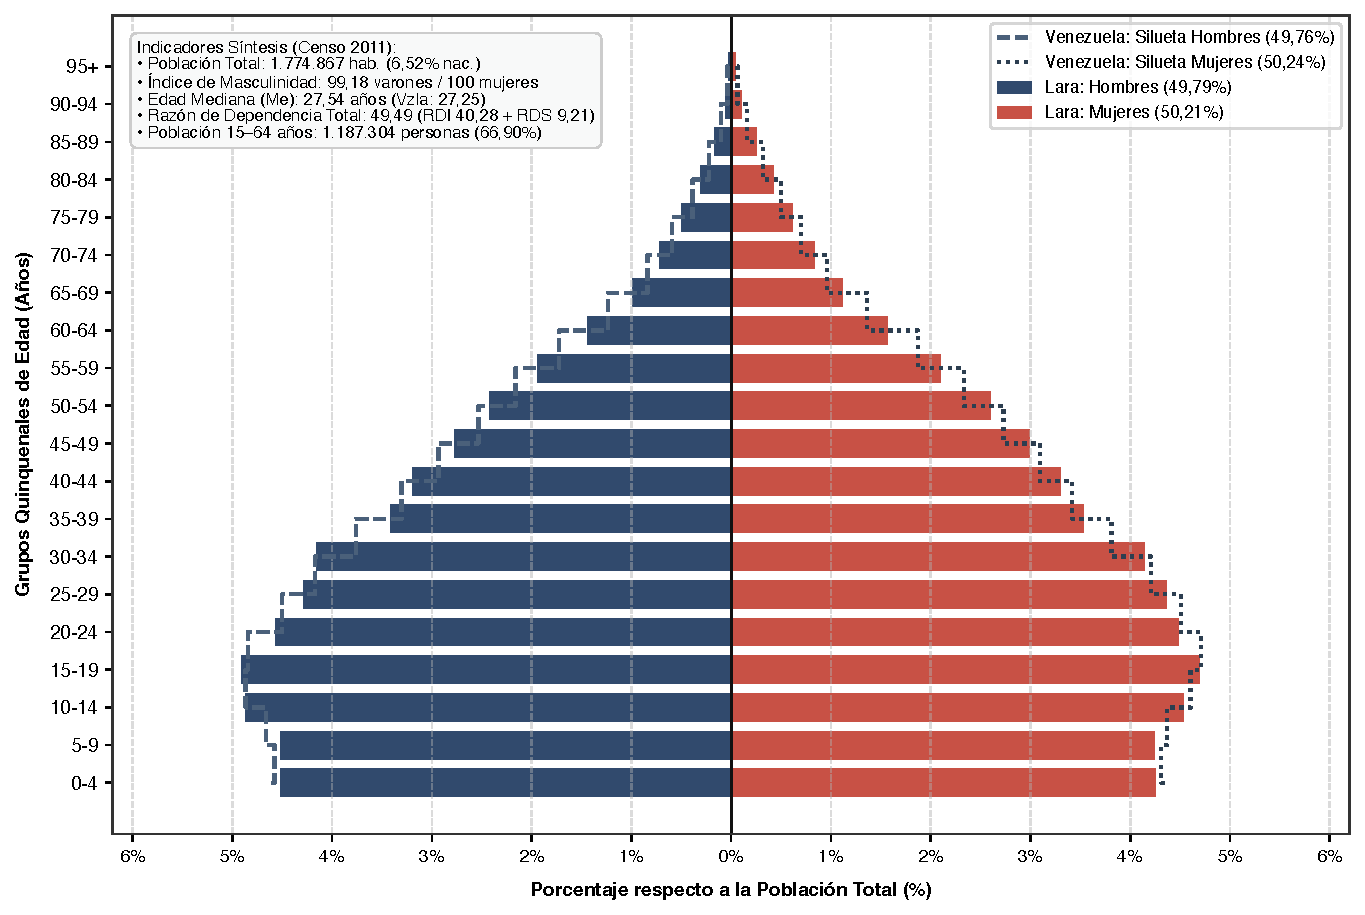
\includegraphics[width=0.88\textwidth]{fig_lara_1.pdf}
    \label{fig:piramide}
    \par\medskip\noindent\raggedright \small \textit{Nota.} Fuente: Tabulados censales del Estado Lara 2011 (I.N.E.). Relación de masculinidad calculada como $IM = (\text{Hombres} / \text{Mujeres}) \times 100$. La silueta escalonada representa la población de Venezuela ($N = 27.227.930$).
\end{figure}

La pirámide quinquenal (Cuadro \ref{tab:piramide_quinquenal} y Figura \ref{fig:piramide}) expone la contracción de la base y la erosión juvenil del cuerpo intermedio. Los tramos de 0 a 4 años (155.691 personas; 8,77\%) y de 5 a 9 años (155.634 niños; 8,77\%) quedan por debajo de los efectivos de 10 a 14 años (166.892 jóvenes; 9,40\%) y del pico modal de 15 a 19 años (170.435 jóvenes; 9,60\%). Esa caída basal certifica el descenso continuado de los nacimientos conforme la fecundidad se aproxima al reemplazo. En el tramo siguiente se abre una muesca de más de 23.000 efectivos entre 15--19 años (170.435) y 30--34 años (147.294), pasando por 20--24 (160.727) y 25--29 (153.592). Como las probabilidades actuariales de muerte no superan 0,015 por quinquenio en esas edades, la pérdida responde a emigración laboral de adultos jóvenes ante la estrechez industrial de la entidad. En la cúspide, el índice de masculinidad cae de 92,74 en 45--49 años a 71,27 en 80--84 y 55,05 en 95 y más, acumulando un superávit femenino geriátrico.

La edad mediana interpolada sobre el intervalo continuo $[25; 30)$ años ($A_i = 5$) sitúa a Lara en 27,54 años, por encima de los 27,25 años de Venezuela ($+0,29$ años). Ese desplazamiento hacia edades centrales obedece a la caída más temprana de la fecundidad larense y al éxodo de adultos jóvenes en edad reproductiva, anticipando una demanda creciente de atención crónica en las décadas siguientes.

\begin{table}[htbp]
    \centering
    \caption{Grandes Grupos de Edad e Índices de Dependencia y Envejecimiento en Lara y Venezuela (2011)}
    \label{tab:estructura}
    \small
    \begin{tabularx}{\textwidth}{>{\raggedright\arraybackslash}Xrrr}
        \toprule
        \textbf{Indicador Demográfico} & \textbf{Estado Lara} & \textbf{Venezuela} & \textbf{Diferencial} \\
        \midrule
        Menores de 15 años ($P_{0-14}$) & 478.217 (26,94\%) & 7.356.774 (27,02\%) & -0,08 pp \\
        Población Activa Potencial ($P_{15-64}$) & 1.187.304 (66,90\%) & 18.250.657 (67,03\%) & -0,13 pp \\
        Adultos Mayores ($P_{65+}$) & 109.346 (6,16\%) & 1.620.499 (5,95\%) & +0,21 pp \\
        \midrule
        Razón de Dependencia Total ($RD$) & 49,49 & 49,19 & +0,30 pts \\
        Razón de Dependencia Infantil ($RDI$) & 40,28 & 40,31 & -0,03 pts \\
        Razón de Dependencia Senil ($RDS$) & 9,21 & 8,88 & +0,33 pts \\
        Índice de Envejecimiento ($IE$) & 22,87\% & 22,03\% & +0,84 pp \\
        Razón de Reemplazo Activo ($RRP$) & 319,68 & 311,34 & +8,34 pts \\
        Edad Mediana ($Me$) & 27,54 años & 27,25 años & +0,29 años \\
        Índice de Masculinidad Global ($IM$) & 99,18 & 99,10 & +0,08 pts \\
        \bottomrule
    \end{tabularx}
    \par\vspace{2pt}\noindent\raggedright \small \textit{Nota.} Fuente: Tabulados censales del Estado Lara 2011 (I.N.E.). Relación de masculinidad calculada como $IM = (\text{Hombres} / \text{Mujeres}) \times 100$. La población en edad laboral ($\ge 15$ años) totaliza 1.296.650 personas ($1.187.304 + 109.346$).
\end{table}

El perfil de grandes grupos etarios confirma que Lara transita la fase central de su bono demográfico con mayor peso senil que el país (Cuadro \ref{tab:estructura}). La población potencialmente activa de 15 a 64 años alcanza 1.187.304 habitantes (66,90\%, $-0,13$ pp respecto al 67,03\% nacional), frente a 478.217 menores de 15 años (26,94\%, $-0,08$ pp) y 109.346 adultos mayores de 65 años y más (6,16\%, $+0,21$ pp sobre el 5,95\% nacional). Con ello, cada 100 personas potencialmente activas soportan 49,49 dependientes ($RDI = 40,28$ niños y $RDS = 9,21$ adultos mayores), superando en 0,30 puntos la Razón de Dependencia de Venezuela (49,19) exclusivamente por el componente senil ($+0,33$ pts frente a $-0,03$ pts infantil). El Índice de Envejecimiento asciende a 22,87\% ($+0,84$ pp sobre el país) y la Razón de Reemplazo Activo registra 319,68 jóvenes de 15--19 años por cada 100 personas de 60--64 próximas al retiro ($+8,34$ pts sobre Venezuela). Aunque esta configuración reduce transitoriamente la carga de manutención familiar y libera margen para acumular capital humano, su aprovechamiento depende de crear empleo formal antes de que el envejecimiento invierta el cociente entre activos y jubilados.

% ==============================================================================
% SECCIÓN 4: ALFABETISMO Y ESCOLARIDAD DE LA POBLACIÓN
% ==============================================================================
\section{Alfabetismo y Escolaridad de la Población}

En el Estado Lara hay 81.340 personas analfabetas entre los 1.463.542 residentes de 10 años y más ($723.313$ hombres y $740.229$ mujeres), excluidos los 311.325 niños de 0 a 9 años. La tasa general de analfabetismo se sitúa en 5,56\%, superando en 0,64 puntos porcentuales el promedio venezolano (4,92\%, sobre 1.101.706 iletrados en 22.387.935 habitantes de 10 años y más):
\[
\text{Tasa de Analfabetismo} = \left( \dfrac{\text{Analfabetos } (\ge 10\text{ años})}{\text{Población total } (\ge 10\text{ años})} \right) \times 100 = \dfrac{81.340}{1.463.542} \times 100 = 5{,}56\%
\]

En términos operativos, aproximadamente 6 de cada 100 larenses de 10 años y más ($5,56$) carecen de dominio de la lectoescritura, frente a 1.382.202 alfabetos (94,44\%). Ese exceso de $+0,64$ puntos porcentuales frente a Venezuela no deriva de la cobertura escolar urbana contemporánea, sino de bolsas históricas de exclusión educativa en caseríos agrícolas y semiáridos donde las escuelas unitarias resultaron insuficientes y el trabajo infantojuvenil interrumpió la escolarización primaria.

\begin{table}[htbp]
    \centering
    \caption{Condición de Alfabetismo por Grupos de Edad y Sexo en Residentes de 10 Años en Adelante, Lara, 2011}
    \label{tab:alfabetismo_quinquenal}
    \scriptsize
    \setlength{\tabcolsep}{2.5pt}
    \begin{tabular*}{\textwidth}{@{\extracolsep{\fill}}lrrrrrrrrrrr}
        \toprule
        & \multicolumn{3}{c}{\textbf{Población Alfabeta}} & \multicolumn{3}{c}{\textbf{Población Analfabeta}} & \textbf{Población} & \multicolumn{3}{c}{\textbf{Tasa de Analfabetismo (\%)}} \\
        \cmidrule(lr){2-4} \cmidrule(lr){5-7} \cmidrule(lr){9-11}
        \textbf{Grupo} & \textbf{Hombres} & \textbf{Mujeres} & \textbf{Total} & \textbf{Hombres} & \textbf{Mujeres} & \textbf{Total} & \textbf{Total 10+} & \textbf{\% H} & \textbf{\% M} & \textbf{\% Total} \\
        \midrule
        10--14 & 84.128 & 79.148 & 163.276 & 2.241 & 1.375 & 3.616 & 166.892 & 2,59\% & 1,71\% & 2,17\% \\
        15--19 & 84.725 & 82.185 & 166.910 & 2.400 & 1.125 & 3.525 & 170.435 & 2,75\% & 1,35\% & 2,07\% \\
        20--24 & 78.546 & 78.432 & 156.978 & 2.508 & 1.241 & 3.749 & 160.727 & 3,09\% & 1,56\% & 2,33\% \\
        25--29 & 73.639 & 76.221 & 149.860 & 2.474 & 1.258 & 3.732 & 153.592 & 3,25\% & 1,62\% & 2,43\% \\
        30--34 & 70.811 & 71.880 & 142.691 & 3.034 & 1.569 & 4.603 & 147.294 & 4,11\% & 2,14\% & 3,13\% \\
        35--39 & 57.626 & 60.887 & 118.513 & 3.044 & 1.742 & 4.786 & 123.299 & 5,02\% & 2,78\% & 3,88\% \\
        40--44 & 53.652 & 56.704 & 110.356 & 3.044 & 1.961 & 5.005 & 115.361 & 5,37\% & 3,34\% & 4,34\% \\
        45--49 & 45.991 & 50.534 & 96.525 & 3.294 & 2.611 & 5.905 & 102.430 & 6,68\% & 4,91\% & 5,76\% \\
        50--54 & 39.647 & 42.985 & 82.632 & 3.410 & 3.234 & 6.644 & 89.276 & 7,92\% & 7,00\% & 7,44\% \\
        55--59 & 31.273 & 33.805 & 65.078 & 3.118 & 3.380 & 6.498 & 71.576 & 9,07\% & 9,09\% & 9,08\% \\
        60--64 & 22.742 & 24.480 & 47.222 & 2.822 & 3.270 & 6.092 & 53.314 & 11,04\% & 11,78\% & 11,43\% \\
        65--69 & 14.957 & 16.171 & 31.128 & 2.679 & 3.670 & 6.349 & 37.477 & 15,19\% & 18,50\% & 16,94\% \\
        70--74 & 10.257 & 11.102 & 21.359 & 2.531 & 3.753 & 6.284 & 27.643 & 19,79\% & 25,26\% & 22,73\% \\
        75--79 & 6.652 & 7.480 & 14.132 & 2.187 & 3.348 & 5.535 & 19.667 & 24,74\% & 30,92\% & 28,14\% \\
        80--84 & 3.913 & 4.821 & 8.734 & 1.493 & 2.764 & 4.257 & 12.991 & 27,62\% & 36,44\% & 32,77\% \\
        85--89 & 2.010 & 2.633 & 4.643 & 972 & 1.855 & 2.827 & 7.470 & 32,60\% & 41,33\% & 37,84\% \\
        90--94 & 683 & 971 & 1.654 & 407 & 902 & 1.309 & 2.963 & 37,34\% & 48,16\% & 44,18\% \\
        95 y más & 196 & 315 & 511 & 207 & 417 & 624 & 1.135 & 51,36\% & 56,97\% & 54,98\% \\
        \midrule
        \textbf{Total 10+} & \textbf{681.448} & \textbf{700.754} & \textbf{1.382.202} & \textbf{41.865} & \textbf{39.475} & \textbf{81.340} & \textbf{1.463.542} & \textbf{5,79\%} & \textbf{5,33\%} & \textbf{5,56\%} \\
        \bottomrule
    \end{tabular*}
    \par\vspace{2pt}\noindent\raggedright \scriptsize \textit{Nota.} Fuente: Censo 2011 para el Estado Lara (I.N.E.), procesamiento REDATAM+SP. Cada tasa de analfabetismo específica por sexo ($\text{\% H}$ y $\text{\% M}$) divide a los analfabetos del sexo respectivo entre la suma de alfabetos más analfabetos de ese mismo sexo y grupo etario ($N_{x,5}^s = \text{Alfabetos}_{x,5}^s + \text{Analfabetos}_{x,5}^s$). En el agregado $\ge 10$ años ($1.463.542$ residentes, excluidos $311.325$ menores de 10 años): $41.865 / 723.313 = 5{,}79\%$ en hombres, $39.475 / 740.229 = 5{,}33\%$ en mujeres y $81.340 / 1.463.542 = 5{,}56\%$ total.
\end{table}

\begin{figure}[htbp]
    \centering
    \caption{Trayectoria Generacional del Alfabetismo y Brecha Territorial en Lara (Censo 2011)}
    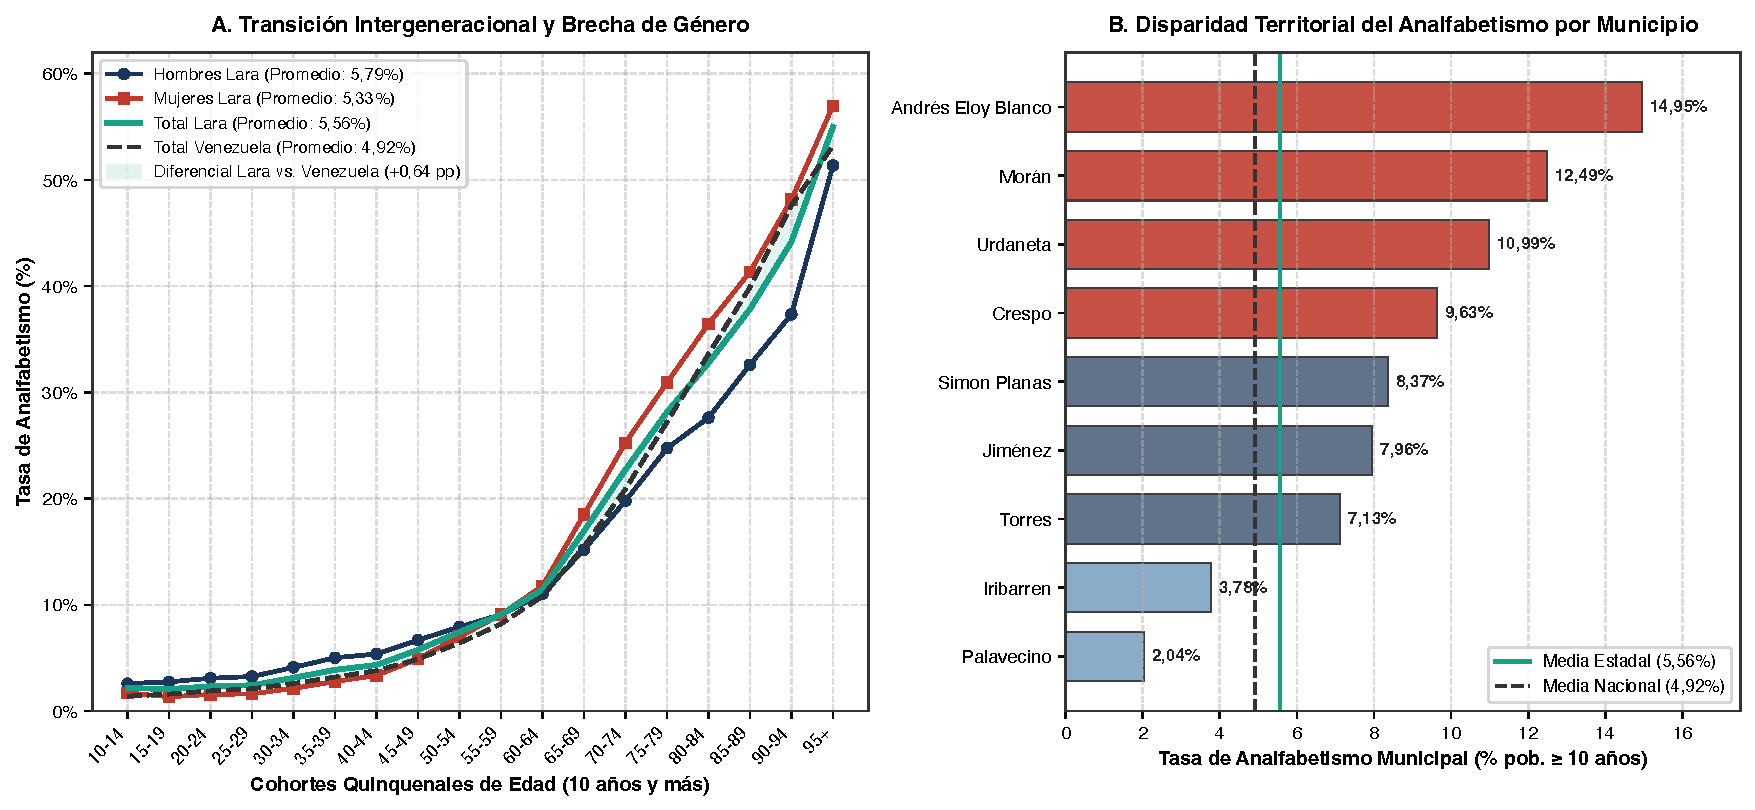
\includegraphics[width=0.88\textwidth]{fig_lara_2.pdf}
    \label{fig:educacion}
    \par\medskip\noindent\raggedright \small \textit{Nota.} Fuente: Tabulados censales del Estado Lara 2011 (I.N.E.). Universo de $1.463.542$ residentes de 10 años y más en Lara y $22.387.935$ en Venezuela.
\end{figure}

La serie por cohortes (Cuadro \ref{tab:alfabetismo_quinquenal} y Figura \ref{fig:educacion}) muestra una contracción generacional severa del analfabetismo acompañada de una inversión completa de la brecha por sexo. La expansión de la educación básica durante la segunda mitad del siglo XX comprimió la privación letrada por debajo del 2,50\% entre los 10 y 29 años (2,17\% en 10--14; 2,07\% en 15--19; 2,33\% en 20--24; 2,43\% en 25--29). En las cohortes nacidas antes de 1950, la tasa escala de 16,94\% en 65--69 años a 28,14\% en 75--79 y alcanza 54,98\% desde los 95 años por la exclusión rural de inicios del siglo XX. Desde los 55 años hacia atrás la ventaja escolar cambia de signo: en 75--79 años el analfabetismo femenino (30,92\%) supera al masculino (24,74\%) porque las familias campesinas priorizaban la escolarización mínima de los varones, mientras que en todas las cohortes menores de 55 años las mujeres exhiben menor analfabetismo (1,35\% frente a 2,75\% en 15--19 años; promedio global de 5,33\% frente a 5,79\%) debido a la deserción masculina temprana hacia faenas agrícolas y oficios manuales. En el mapa municipal (Figura \ref{fig:educacion}, Panel B), esa brecha separa netamente a Palavecino (2,04\%) e Iribarren (3,78\%)—ambos por debajo del 4,92\% nacional—frente a Crespo (9,63\%), Urdaneta (10,99\%), Morán (12,49\%) y Andrés Eloy Blanco (14,95\%). El trabajo infantojuvenil en cafetales, cañaverales y conucos explica que el rezago rural triplique o cuadruplique la tasa metropolitana.

\begin{table}[htbp]
    \centering
    \caption{Nivel Educativo de la Población Adulta ($\ge 25$ Años) según Sexo en Lara (2011)}
    \label{tab:instruccion}
    \small
    \begin{tabularx}{\textwidth}{>{\raggedright\arraybackslash}Xrrrrrr}
        \toprule
        \textbf{Nivel de Instrucción} & \textbf{Hombres} & \textbf{\% (H)} & \textbf{Mujeres} & \textbf{\% (M)} & \textbf{Total} & \textbf{\% Total} \\
        \midrule
        Ninguno & 33.984 & 7,34\% & 34.381 & 6,84\% & 68.365 & 7,08\% \\
        Primaria & 158.598 & 34,25\% & 139.435 & 27,75\% & 298.033 & 30,87\% \\
        Secundaria & 175.917 & 37,99\% & 185.285 & 36,88\% & 361.202 & 37,41\% \\
        Técnico Superior (TSU) & 20.816 & 4,50\% & 28.746 & 5,72\% & 49.562 & 5,13\% \\
        Universitario & 59.894 & 12,93\% & 102.169 & 20,34\% & 162.063 & 16,79\% \\
        No sabe o No declarado & 13.852 & 2,99\% & 12.411 & 2,47\% & 26.263 & 2,72\% \\
        \midrule
        \textbf{Total Población $\ge$ 25} & \textbf{463.061} & \textbf{100,00\%} & \textbf{502.427} & \textbf{100,00\%} & \textbf{965.488} & \textbf{100,00\%} \\
        \bottomrule
    \end{tabularx}
    \par\vspace{2pt}\noindent\raggedright \small \textit{Nota.} Fuente: Tabulados censales del Estado Lara 2011 (I.N.E.). Los porcentajes por columna dividen cada categoría entre el total de adultos de 25 años y más del sexo respectivo ($463.061$ hombres, $502.427$ mujeres y $965.488$ en total). La educación superior agregada (TSU más Universitario) suma $80.710$ hombres ($17{,}43\%$), $130.915$ mujeres ($26{,}06\%$) y $211.625$ adultos ($21{,}92\%$).
\end{table}

La superioridad académica femenina se amplifica en la educación terciaria de los 965.488 adultos de 25 años y más (Cuadro \ref{tab:instruccion}). Las mujeres representan el 63,04\% de los graduados universitarios (102.169 tituladas frente a 59.894 hombres) y el 26,06\% de todas las mujeres adultas posee credencial superior completa (TSU o universitaria, 130.915 personas), frente al 17,43\% de los varones (80.710 personas), cuya mayor inserción temprana en agricultura, construcción y comercio informal prescinde de titulación formal, mientras el sector terciario formal urbano exige credenciales académicas para el ingreso femenino. Los 26.263 registros sin declaración (2,72\%) corresponden principalmente a respuestas incompletas de hogares periféricos o población de edad avanzada y no alteran la brecha superior femenina, aunque su aprovechamiento productivo queda restringido por la baja demanda técnica de la economía regional.

% ==============================================================================
% SECCIÓN 5: RÉGIMEN CONYUGAL Y NUPCIALIDAD
% ==============================================================================
\section{Régimen Conyugal y Nupcialidad}

En Lara la cohabitación consensual supera al matrimonio civil. Entre los 1.289.325 adultos de 15 años y más con declaración válida, 346.318 personas conviven en unión libre (26,86\%) frente a 305.232 casadas civilmente (23,67\%), fijando una razón de 1,13 uniones consensuales por cada matrimonio formal.

Antes de calcular las proporciones adultas conviene acotar el universo censal (Cuadro \ref{tab:conyugal_edad_sexo}). De los 1.463.542 residentes de 10 años y más, 1.455.613 declararon válidamente su estado conyugal ($718.886$ hombres y $736.727$ mujeres), excluyéndose 7.929 casos sin respuesta ($604$ en edades menores de 15 años y $7.325$ en adultos de 15 años y más). Para evitar que la soltería casi universal del tramo 12--14 años (165.663 solteros sobre 166.288 declarantes, aunque ya aparecen 446 niñas unidas y 91 casadas frente a 65 varones unidos) distorsione el régimen nupcial adulto, se separa ese subtotal inicial dejando exactamente 1.289.325 adultos evaluados (Cuadro \ref{tab:conyugal_colapsada}).

\begin{table}[htbp]
    \centering
    \caption{Estado Conyugal por Grupos Etarios y Sexo a Partir de los 12 Años en Lara (2011)}
    \label{tab:conyugal_edad_sexo}
    \scriptsize
    \setlength{\tabcolsep}{2.5pt}
    \resizebox{\textwidth}{!}{%
    \begin{tabular}{lrrrrrrrrrrrrrr}
        \toprule
        & \multicolumn{7}{c}{\textbf{Hombres}} & \multicolumn{7}{c}{\textbf{Mujeres}} \\
        \cmidrule(lr){2-8} \cmidrule(lr){9-15}
        \textbf{Grupo} & \textbf{Unido} & \textbf{Casado} & \textbf{Soltero} & \textbf{Sep.} & \textbf{Div.} & \textbf{Viudo} & \textbf{Total H.} & \textbf{Unida} & \textbf{Casada} & \textbf{Soltera} & \textbf{Sep.} & \textbf{Div.} & \textbf{Viuda} & \textbf{Total M.} \\
        \midrule
        12--14 años & 65 & 0 & 86.152 & 4 & 0 & 0 & 86.221 & 446 & 91 & 79.511 & 17 & 0 & 2 & 80.067 \\
        15--19 & 3.194 & 400 & 82.630 & 52 & 19 & 11 & 86.306 & 10.665 & 1.222 & 70.300 & 393 & 13 & 43 & 82.636 \\
        20--24 & 17.464 & 3.338 & 58.906 & 378 & 44 & 27 & 80.157 & 24.881 & 6.754 & 45.862 & 1.356 & 90 & 167 & 79.110 \\
        25--29 & 27.049 & 10.739 & 36.625 & 798 & 171 & 36 & 75.418 & 29.393 & 14.707 & 30.124 & 2.196 & 351 & 285 & 77.056 \\
        30--34 & 28.929 & 17.113 & 25.191 & 1.413 & 532 & 85 & 73.263 & 27.623 & 19.645 & 21.631 & 2.814 & 978 & 410 & 73.101 \\
        35--39 & 23.129 & 18.192 & 16.603 & 1.510 & 799 & 140 & 60.373 & 21.998 & 19.169 & 16.113 & 3.005 & 1.533 & 629 & 62.447 \\
        40--44 & 20.035 & 19.038 & 14.251 & 1.744 & 1.123 & 276 & 56.467 & 18.424 & 19.618 & 14.109 & 3.207 & 2.178 & 953 & 58.489 \\
        45--49 & 16.212 & 18.088 & 11.429 & 1.744 & 1.266 & 352 & 49.091 & 14.531 & 18.629 & 12.413 & 3.368 & 2.533 & 1.528 & 53.002 \\
        50--54 & 12.989 & 16.848 & 9.456 & 1.714 & 1.330 & 566 & 42.903 & 10.396 & 16.428 & 10.887 & 3.105 & 2.964 & 2.306 & 46.086 \\
        55--59 & 9.054 & 14.948 & 6.964 & 1.386 & 1.192 & 716 & 34.260 & 6.625 & 13.485 & 8.160 & 2.600 & 2.907 & 3.328 & 37.105 \\
        60--64 & 6.216 & 11.430 & 4.838 & 1.060 & 956 & 979 & 25.479 & 3.970 & 9.571 & 5.977 & 1.774 & 2.252 & 4.152 & 27.696 \\
        65--69 & 3.799 & 8.035 & 3.361 & 683 & 597 & 1.097 & 17.572 & 2.204 & 6.293 & 4.231 & 1.130 & 1.352 & 4.557 & 19.767 \\
        70--74 & 2.387 & 5.798 & 2.443 & 447 & 417 & 1.250 & 12.742 & 1.295 & 3.898 & 3.228 & 679 & 806 & 4.895 & 14.801 \\
        75--79 & 1.464 & 3.996 & 1.649 & 272 & 228 & 1.206 & 8.815 & 703 & 2.300 & 2.360 & 400 & 449 & 4.575 & 10.787 \\
        80--84 & 734 & 2.264 & 993 & 137 & 112 & 1.136 & 5.376 & 299 & 1.106 & 1.683 & 234 & 268 & 3.946 & 7.536 \\
        85--89 & 333 & 1.133 & 563 & 72 & 73 & 791 & 2.965 & 130 & 432 & 1.052 & 119 & 122 & 2.606 & 4.461 \\
        90--94 & 101 & 343 & 221 & 19 & 18 & 377 & 1.079 & 49 & 136 & 476 & 32 & 44 & 1.120 & 1.857 \\
        95 y más & 29 & 100 & 83 & 10 & 5 & 172 & 399 & 14 & 36 & 204 & 19 & 16 & 434 & 723 \\
        \midrule
        \textbf{Subtotal (15 años y más)} & \textbf{173.118} & \textbf{151.803} & \textbf{276.206} & \textbf{13.439} & \textbf{8.882} & \textbf{9.217} & \textbf{632.665} & \textbf{173.200} & \textbf{153.429} & \textbf{248.810} & \textbf{26.431} & \textbf{18.856} & \textbf{35.934} & \textbf{656.660} \\
        \textbf{Total (12 años y más)} & \textbf{173.183} & \textbf{151.803} & \textbf{362.358} & \textbf{13.443} & \textbf{8.882} & \textbf{9.217} & \textbf{718.886} & \textbf{173.646} & \textbf{153.520} & \textbf{328.321} & \textbf{26.448} & \textbf{18.856} & \textbf{35.936} & \textbf{736.727} \\
        \bottomrule
    \end{tabular}%
    }
    \par\vspace{2pt}\noindent\raggedright \scriptsize \textit{Nota.} Fuente: Base de datos censal del Estado Lara 2011 (I.N.E.). Sobre $1.463.542$ residentes de 10 años y más ($166.892$ menores de 15 años y $1.296.650$ de 15 años y más), declararon válidamente su estado conyugal $1.455.613$ personas ($166.288$ en el tramo inicial $12\text{--}14$ años y $1.289.325$ en el subtotal de 15 años y más), excluyéndose $7.929$ casos sin declaración ($604$ menores de 15 años y $7.325$ de 15 años y más).
\end{table}

\begin{table}[htbp]
    \centering
    \caption{Categorías Conyugales Agregadas en la Población Adulta ($\ge 15$ Años) de Lara (2011)}
    \label{tab:conyugal_colapsada}
    \small
    \setlength{\tabcolsep}{3pt}
    \begin{tabularx}{\textwidth}{>{\raggedright\arraybackslash}Xrrrrrrrr}
        \toprule
        \textbf{Sexo ($\ge 15$ años)} & \textbf{Solteros} & \textbf{\% Solt.} & \textbf{Cas.-Unid.} & \textbf{\% Cas.-Un.} & \textbf{Disueltos} & \textbf{\% Dis.} & \textbf{Total} & \textbf{\% Total} \\
        \midrule
        Hombres & 276.206 & 43,66\% & 324.921 & 51,36\% & 31.538 & 4,98\% & 632.665 & 100,00\% \\
        Mujeres & 248.810 & 37,89\% & 326.629 & 49,74\% & 81.221 & 12,37\% & 656.660 & 100,00\% \\
        \midrule
        \textbf{Total Estado Lara} & \textbf{525.016} & \textbf{40,72\%} & \textbf{651.550} & \textbf{50,53\%} & \textbf{112.759} & \textbf{8,75\%} & \textbf{1.289.325} & \textbf{100,00\%} \\
        \bottomrule
    \end{tabularx}
    \par\vspace{2pt}\noindent\raggedright \small \textit{Nota.} Fuente: Elaboración propia a partir de microdatos censales 2011 (I.N.E.), excluidos $7.325$ casos adultos sin declaración. Cierre exacto desde el subtotal $\ge 15$ años del Cuadro \ref{tab:conyugal_edad_sexo}: \textit{Cas.-Unid.} suma $346.318$ unidos ($173.118$ H + $173.200$ M; $26{,}86\%$) y $305.232$ casados ($151.803$ H + $153.429$ M; $23{,}67\%$), con razón $1{,}13$ uniones por matrimonio; \textit{Disueltos} suma $39.870$ separados ($13.439$ H + $26.431$ M; $3{,}09\%$), $27.738$ divorciados ($8.882$ H + $18.856$ M; $2{,}15\%$) y $45.151$ viudos ($9.217$ H + $35.934$ M; $3{,}50\%$).
\end{table}

\begin{figure}[htbp]
    \centering
    \caption{Distribución Conyugal y Pauta de Emparejamiento por Edad en Lara (2011)}
    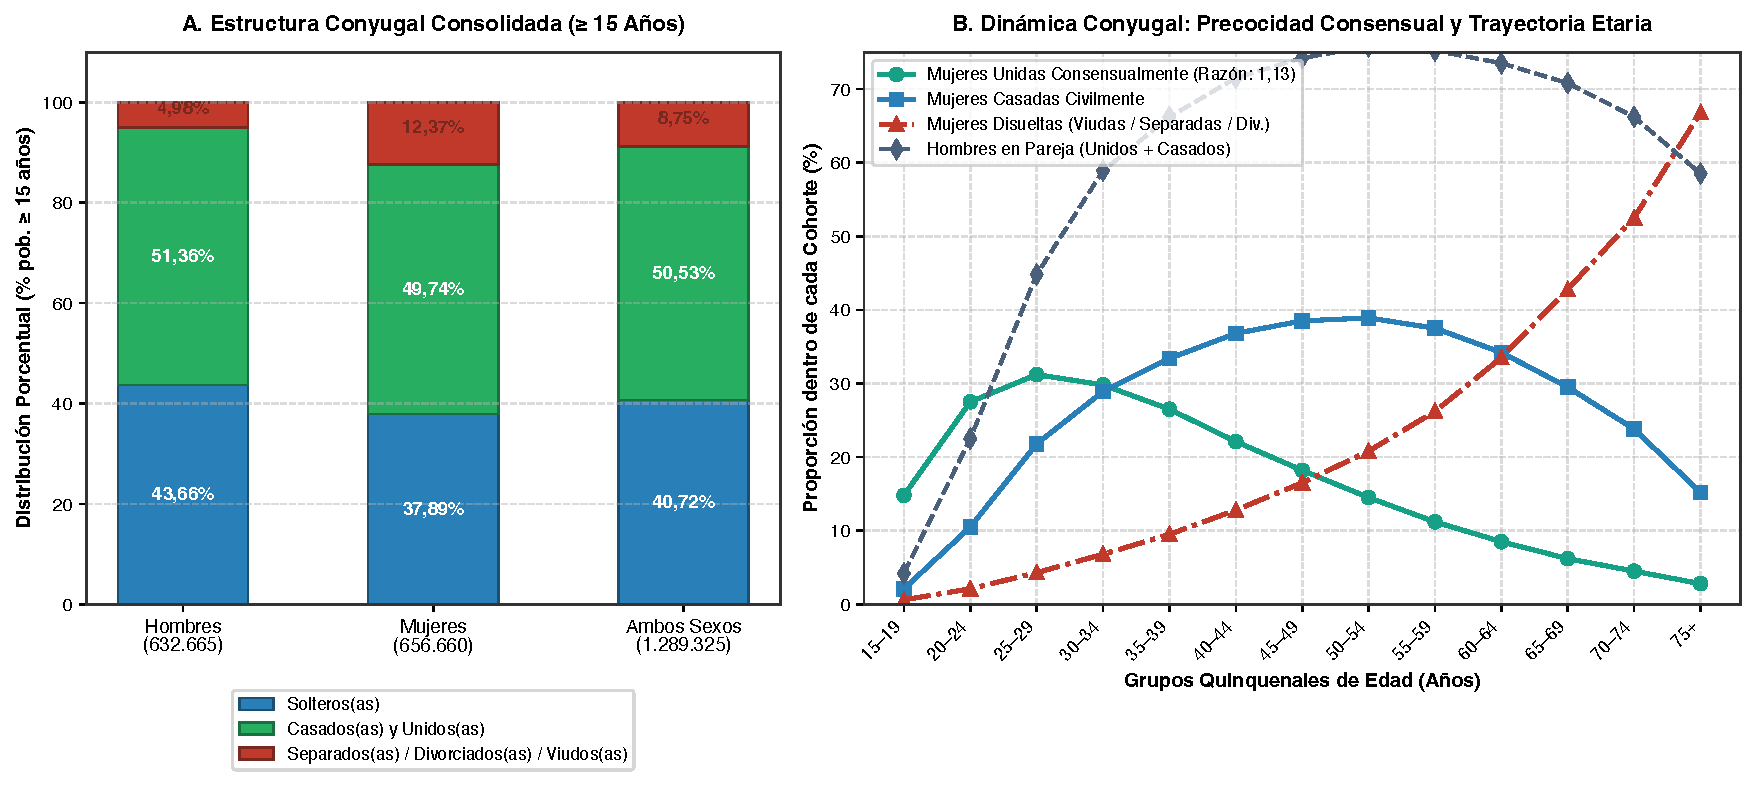
\includegraphics[width=0.88\textwidth]{fig_lara_3.pdf}
    \label{fig:conyugal}
    \par\medskip\noindent\raggedright \small \textit{Nota.} Fuente: Tabulados censales del Estado Lara 2011 (I.N.E.). Panel A: composición por categorías colapsadas en $\ge 15$ años ($1.289.325$ declarantes); Panel B: trayectoria etaria por cohorte quinquenal.
\end{figure}

El calendario conyugal (Cuadro \ref{tab:conyugal_colapsada} y Figura \ref{fig:conyugal}) refleja trayectorias divergentes por edad y sexo. Mientras la soltería retiene al 40,72\% de los adultos (43,66\% en hombres frente a 37,89\% en mujeres), la unión conyugal activa (50,53\%) comienza de forma precoz bajo modalidad consensual en la cohorte de 20 a 24 años, donde 24.881 mujeres viven unidas de hecho frente a 6.754 casadas civilmente (razón de 3,68 uniones por matrimonio), debido a la menor barrera patrimonial y contractual de la cohabitación en hogares de ingresos informales. El matrimonio civil solo pasa a dominar en edades maduras entre los 35 y 54 años, por consolidación patrimonial y formalización tardía de vínculos previos. En el extremo opuesto, las mujeres concentran el 72,03\% de las uniones disueltas (81.221 mujeres o 12,37\%, frente a 31.538 hombres o 4,98\%). La sobremortalidad masculina genera una brecha de viudez de 35.934 mujeres frente a 9.217 hombres (66,80\% en mujeres mayores de 75 años), a la vez que la menor probabilidad de reemparejamiento femenino tras la separación duplica la cantidad de mujeres separadas (26.431 frente a 13.439) y divorciadas (18.856 frente a 8.882).

Esta estructura nupcial acelera la fisión de hogares y agrava el déficit urbano en Barquisimeto y Cabudare. El ingreso temprano a la cohabitación consensual en edades de 20 a 29 años junto al 40,72\% de soltería adulta fragmentan los arreglos domésticos, multiplicando la demanda de viviendas independientes y elevando la carga de conexiones sobre el acueducto metropolitano Dos Cerritos--Atarigua, las redes cloacales y las subestaciones eléctricas. Dado que el 42,00\% de la población ocupada percibe ingresos informales sin acceso al crédito hipotecario bancario, el excedente de nuevos hogares deriva en hacinamiento intrafamiliar, presión alcista sobre alquileres en Palavecino y expansión de asentamientos no consolidados al oeste de Barquisimeto, particularmente en la parroquia Juan de Villegas (sector Guerrera Ana Soto).

% ==============================================================================
% SECCIÓN 6: INSERCIÓN LABORAL Y ESTRUCTURA OCUPACIONAL
% ==============================================================================
\section{Inserción Laboral y Estructura Ocupacional}

Dos de cada cinco ocupados en Lara trabajan en el sector informal (42,00\%, 294.508 personas). La incapacidad de la manufactura regional para absorber la oferta creciente del bono demográfico empuja al excedente activo hacia el comercio y los servicios de subsistencia.

La cuantificación de la fuerza de trabajo exige conciliar dos instrumentos estadísticos con cobertura distinta (Cuadro \ref{tab:laboral_resumen}). De los 1.463.542 residentes de 10 años y más, los 166.892 jóvenes de 10 a 14 años cursan educación básica y media fuera del mercado laboral, delimitando en el Censo 2011 una Población en Edad de Trabajar ($\text{PET} \ge 15$ años) de 1.296.650 habitantes ($638.485$ hombres y $658.165$ mujeres). En la enumeración censal directa, la Población Económicamente Activa ($\text{PEA}$) suma 794.846 personas ($TAE = 61,30\%$), desagregadas en 731.258 ocupados ($TO = 92,00\%$) y 63.588 desocupados ($TD = 8,00\%$), frente a 501.804 inactivos ($\text{PNEA}$, 38,70\%). El relevamiento muestral de la Encuesta de Hogares por Muestreo (EHM), en cambio, restringido a viviendas particulares habitadas y medido con criterios de semana de referencia más estrictos sobre disponibilidad laboral, calibra la $\text{PET}$ operativa en 1.290.760 personas ($-5.890$ frente al censo por exclusión de viviendas colectivas y ajuste muestral), reduciendo la $\text{PEA}$ a 757.245 activos ($TAE = 58,67\%$; Tasa Bruta de Actividad de 42,66\% sobre la población total) y elevando la $\text{PNEA}$ a 533.515 personas ($41,33\%$), con 701.209 ocupados ($TO = 92,60\%$) y 56.036 desocupados ($TD = 7,40\%$). En ambas fuentes se repite el mismo gradiente etario: la participación alcanza su máximo entre los 25 y 44 años ($79,98\%$) y la desocupación golpea con fuerza a los jóvenes de 15 a 24 años ($13,96\%$ en el censo; $17,20\%$ en la serie muestral de la Figura \ref{fig:laboral}), quienes chocan contra una absorción laboral estrecha.

\begin{table}[htbp]
    \centering
    \caption{Estructura de la Fuerza de Trabajo, Ocupación y Desocupación en Lara (2011)}
    \label{tab:laboral_resumen}
    \scriptsize
    \setlength{\tabcolsep}{3pt}
    \begin{tabular*}{\textwidth}{@{\extracolsep{\fill}}lrrrrrrrr}
        \toprule
        \multicolumn{9}{l}{\textbf{Panel A. Fuerza de Trabajo por Grupos de Edad en Lara (Censo 2011 y Calibración EHM)}} \\
        \midrule
        \textbf{Grupo de Edad} & \textbf{PET ($\ge 15$)} & \textbf{PEA (Activos)} & \textbf{Ocupados} & \textbf{Desocupados} & \textbf{PNEA (Inact.)} & \textbf{TAE (\%)} & \textbf{TO (\%)} & \textbf{TD (\%)} \\
        \midrule
        15--24 años & 331.162 & 149.255 & 128.412 & 20.843 & 181.907 & 45,07\% & 86,04\% & 13,96\% \\
        25--44 años & 539.546 & 431.542 & 401.218 & 30.324 & 108.004 & 79,98\% & 92,97\% & 7,03\% \\
        45--64 años & 316.596 & 196.153 & 184.465 & 11.688 & 120.443 & 61,96\% & 94,04\% & 5,96\% \\
        65 y más años & 109.346 & 17.896 & 17.163 & 733 & 91.450 & 16,37\% & 95,90\% & 4,10\% \\
        \midrule
        \textbf{Total Estado Lara (Censo)} & \textbf{1.296.650} & \textbf{794.846} & \textbf{731.258} & \textbf{63.588} & \textbf{501.804} & \textbf{61,30\%} & \textbf{92,00\%} & \textbf{8,00\%} \\
        Total Lara (EHM) & 1.290.760 & 757.245 & 701.209 & 56.036 & 533.515 & 58,67\% & 92,60\% & 7,40\% \\
        \bottomrule
    \end{tabular*}
    \par\vspace{6pt}
    \begin{tabularx}{\textwidth}{>{\raggedright\arraybackslash}p{2.3cm}>{\raggedright\arraybackslash}Xrrrrr}
        \toprule
        \multicolumn{7}{l}{\textbf{Panel B. Distribución de los Ocupados por Macro-Sectores y Condición de Formalidad (EHM, 2011)}} \\
        \midrule
        \textbf{Macro-Sector} & \textbf{Rama de Actividad Económica} & \textbf{Ocupados} & \textbf{\% Ocup.} & \textbf{Formal} & \textbf{Informal} & \textbf{\% Inf.} \\
        \midrule
        Sector Primario & Agricultura bajo riego, cañicultura, café y ganadería & 98.169 & 14,00\% & 35.341 & 62.828 & 64,00\% \\
        Sector Secundario & Manufactura fabril (Iribarren) y Construcción civil & 140.242 & 20,00\% & 78.536 & 61.706 & 44,00\% \\
        Sector Terciario & Comercio mayorista/al detal (MERCABAR) y Servicios & 462.798 & 66,00\% & 292.824 & 169.974 & 36,73\% \\
        \midrule
        \textbf{Total Ramas} & \textbf{Totalidad de Ramas Económicas Integradas} & \textbf{701.209} & \textbf{100,00\%} & \textbf{406.701} & \textbf{294.508} & \textbf{42,00\%} \\
        \bottomrule
    \end{tabularx}
    \par\vspace{2pt}\noindent\raggedright \scriptsize \textit{Nota.} Fuente: Conciliación propia de microdatos del Censo 2011 y de la Encuesta de Hogares por Muestreo EHM (I.N.E., Estado Lara). El Panel A muestra el desglose etario censal exhaustivo ($\text{PET} = 1.296.650$) frente a la calibración muestral de viviendas particulares en la EHM ($\text{PET} = 1.290.760$), sobre cuyo universo de $701.209$ ocupados se desagregan los macro-sectores y la formalidad del Panel B ($406.701$ formales, $58{,}00\%$; $294.508$ informales, $42{,}00\%$).
\end{table}

La composición interna de la EHM revela la fragilidad cualitativa de la inserción laboral. Dentro de los 701.209 ocupados, los asalariados reúnen 420.725 puestos (60,00\%) entre 139.540 empleados públicos con cobertura previsional (19,90\%) y 281.185 privados (40,10\%), mientras los ocupados por cuenta propia abarcan 245.423 personas (35,00\%) en comercio ambulante y agricultura campesina sin seguridad social, quedando apenas 35.061 empleadores (5,00\%). En la desocupación (56.036 personas; 7,40\%) y la inactividad (533.515 personas; 41,33\%), 48.751 cesantes (87,00\%) y 7.285 aspirantes primerizos (13,00\%) reflejan el taponamiento de entrada juvenil, frente a 245.417 personas en quehaceres del hogar (46,00\%; con sobrecarga femenina), 186.730 estudiantes (35,00\%), 74.692 jubilados (14,00\%) y 26.676 incapacitados permanentes (5,00\%).

\begin{figure}[htbp]
    \centering
    \caption{Composición Ocupacional por Ramas y Condición de Formalidad en Lara (2011)}
    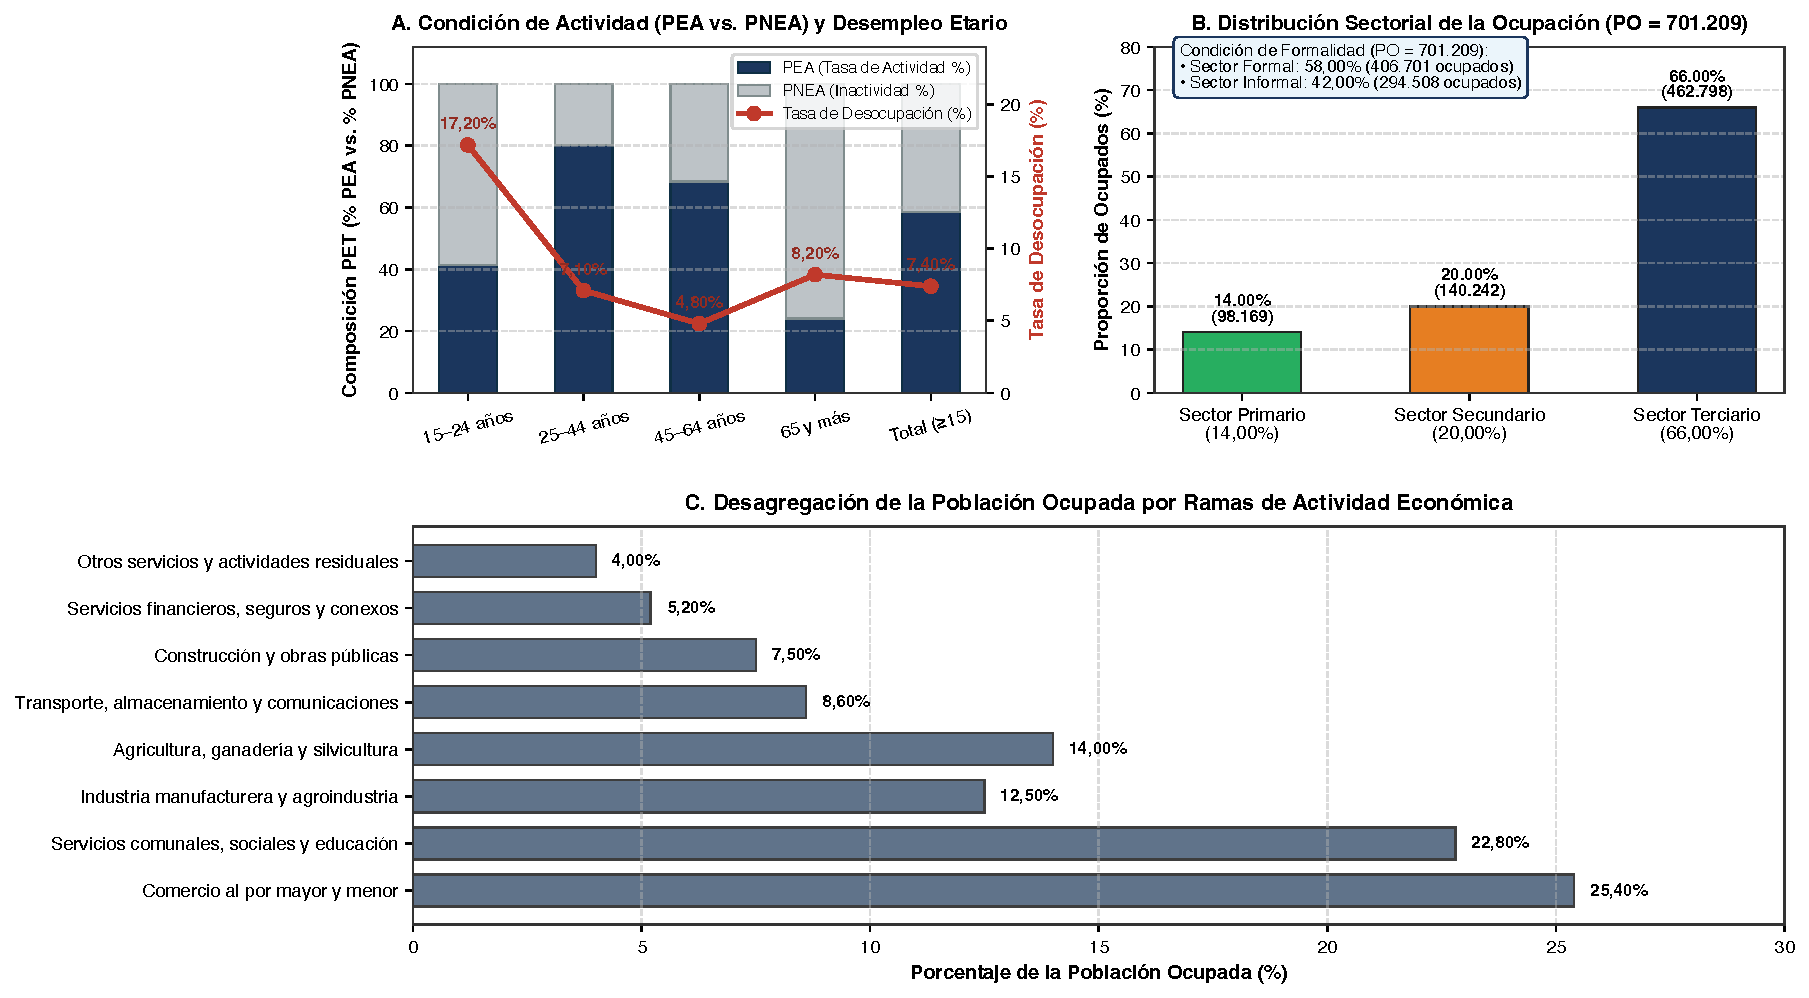
\includegraphics[width=0.90\textwidth]{fig_lara_4.pdf}
    \label{fig:laboral}
    \par\medskip\noindent\raggedright \small \textit{Nota.} Fuente: Tabulados laborales de 2011 (I.N.E., Censo y EHM). Cálculos propios.
\end{figure}

El desglose sectorial y el nivel de calificación exponen dos formas simultáneas de subempleo (Cuadro \ref{tab:laboral_resumen}, Panel B y Figura \ref{fig:laboral}). En el sector primario (98.169 ocupados; 14,00\%, con 64,00\% de informalidad), la rotación de suelos y el racionamiento hídrico en Quíbor junto al fin de la zafra cañicultora en Morán someten a los jornaleros a subempleo visible de menos de 35 horas semanales involuntarias. Ese déficit horario se reproduce en las cuadrillas discontinuas de construcción en Barquisimeto, dentro del 20,00\% secundario (140.242 ocupados con 44,00\% de informalidad). Al mismo tiempo, el sector terciario absorbe 462.798 ocupados (66,00\%; 36,73\% informal), liderado por el comercio mayorista y minorista (25,40\%) y los servicios comunales y educativos (22,80\%). Aplicando la cuota de 21,92\% de educación superior adulta del Cuadro \ref{tab:instruccion} al contingente ocupado (153.700 profesionales TSU o universitarios), miles de graduados quedan atrapados en subempleo invisible dentro del comercio informal y los servicios de baja remuneración ante la estrechez fabril (12,50\%). Esa descalificación afecta especialmente a las mujeres tituladas, dilapidando la inversión educativa acumulada durante el bono demográfico.

% ==============================================================================
% SECCIÓN 7: COMPONENTES DEL CAMBIO DEMOGRÁFICO Y PROYECCIÓN 2011-2016
% ==============================================================================
\section{Componentes del Cambio Demográfico y Proyección 2011--2016}

Lara dejó de ser un polo receptor neto de migración interna. El balance acumulado de toda la vida en 2011 arroja un saldo migratorio neto negativo de $-45.652$ habitantes ($-25,72\text{‰}$), revirtiendo la atracción demográfica que impulsó a Barquisimeto hasta finales del siglo XX.

Los registros censales contabilizan 1.552.935 nativos nacidos y residentes en la entidad (87,50\% redondeado del total estadal, 87,496\% exacto; los restantes 38.738 residentes corresponden a nacidos en el exterior o sin entidad declarada) frente a 183.194 inmigrantes procedentes de otros estados ($103,22\text{‰}$) y 228.846 nativos larenses empadronados fuera de Lara ($128,94\text{‰}$), sobre un denominador común de 1.774.867 habitantes (Cuadro \ref{tab:migracion}). Sobre una movilidad bruta acumulada de 412.040 desplazamientos, el Índice de Eficiencia Migratoria desciende a $-11,08\%$ y la razón entre inmigrantes y emigrantes cae a 0,8005 (80 ingresos por cada 100 salidas). Aunque la migración de toda la vida mezcla desplazamientos de distintas décadas sin precisar la fecha exacta de traslado, su signo negativo concuerda con la muesca observada entre los 20 y 34 años en la pirámide (Cuadro \ref{tab:piramide_quinquenal}), confirmando el drenaje neto de adultos jóvenes calificados hacia mercados laborales externos ante la limitada industrialización estadal.

\begin{table}[htbp]
    \centering
    \caption{Balance de la Migración Toda la Vida e Intercambio Interestatal en Lara (2011)}
    \label{tab:migracion}
    \small
    \begin{tabularx}{\textwidth}{>{\raggedright\arraybackslash}Xrr}
        \toprule
        \textbf{Concepto e Indicador Migratorio} & \textbf{Valor Absoluto} & \textbf{Tasa e Indicador Relativo} \\
        \midrule
        Población Nativa No Migrante (Nacida y Residente en Lara) & 1.552.935 & 87,49\% de la población total \\
        Inmigrantes Acumulados (Nacidos en otra entidad residentes en Lara) & 183.194 & Tasa Inmigración: 103,22‰ \\
        Emigrantes Acumulados (Nativos de Lara residentes en otra entidad) & 228.846 & Tasa Emigración: 128,94‰ \\
        \midrule
        \textbf{Saldo Migratorio Neto Acumulado} & \textbf{-45.652} & \textbf{Tasa Migración Neta: -25,72‰} \\
        Movilidad Bruta Interna Toda la Vida ($I + E$) & 412.040 & Volumen Bruto de Intercambio \\
        Índice de Eficiencia Migratoria ($\dfrac{\text{Saldo}}{\text{Bruta}} \times 100$) & -11,08\% & Condición: Expulsora Neta \\
        Razón $\dfrac{\text{Inmigrantes}}{\text{Emigrantes}}$ & 0,8005 & 80 inmigrantes por cada 100 emigrantes \\
        \bottomrule
    \end{tabularx}
    \par\vspace{2pt}\noindent\raggedright \small \textit{Nota.} Fuente: Tabulados censales del Estado Lara 2011 (I.N.E.). Todas las tasas dividen entre la población censal total de Lara ($1.774.867$ habitantes). El complemento respecto a $1.774.867$ tras sumar nativos residentes ($1.552.935$ personas; $87{,}50\%$ redondeado) e inmigrantes interestatales ($183.194$ personas; $10{,}32\%$) corresponde a $38.738$ nacidos en el exterior o sin entidad especificada ($2{,}18\%$).
\end{table}

El análisis de la fecundidad exige explicitar dos ajustes censales entre la estructura demográfica general y el módulo reproductivo (Cuadro \ref{tab:fecundidad}). Mientras el vector censal completo del Cuadro \ref{tab:piramide_quinquenal} suma 488.350 Mujeres en Edad Fértil (MEF, 15 a 49 años), el módulo censal con declaración válida de paridez reúne 484.570 MEF, mediando 3.780 mujeres sin declaración de hijos nacidos vivos; de forma análoga, los 31.479 nacidos vivos registrados en 2011 ($TBN = 17,74\text{‰}$ sobre la población total y $TFG = 64,96\text{‰}$ sobre las 484.570 MEF declarantes, o $64,46\text{‰}$ sobre el vector completo) suman 31.217 nacimientos con edad materna declarada más 262 nacimientos con edad materna no declarada redistribuidos en las tasas específicas. La curva reproductiva alcanza su cúspide temprana en 20--24 años ($115,97\text{‰}$, 9.151 nacimientos) y 25--29 años ($107,77\text{‰}$, 8.286), acompañada de una fecundidad adolescente elevada en 15--19 años ($65,06\text{‰}$, 5.372 nacimientos) asociada a las uniones consensuales tempranas y a la deserción escolar en áreas periféricas. Con una suma de tasas específicas de $\sum {}_5f_x = 0,41256$, la Tasa Global de Fecundidad alcanza $\text{TGF} = 5 \times 0,41256 = 2,06$ hijos por mujer (0,35 hijos debajo del promedio nacional de 2,41) y la Tasa Bruta de Reproducción se fija en $R' = 1,01$ hijas por madre, situando a Lara en el límite biológico de reemplazo generacional (2,10 hijos por mujer), mientras la paridez final de la cohorte 45--49 años en 2,86 hijos (con 9,10\% de nuliparidad) refleja la contracción secular del tamaño familiar.

\begin{table}[htbp]
    \centering
    \caption{Fecundidad por Edad, Descendencia Media y Proporción Sin Hijos en Mujeres Larenses (2011)}
    \label{tab:fecundidad}
    \small
    \begin{tabular*}{\textwidth}{@{\extracolsep{\fill}}lrrrrr}
        \toprule
        \textbf{Grupo de Edad} & \textbf{Mujeres (MEF)} & \textbf{Nacidos ($B_x$)} & \textbf{TEF ($f_x$ ‰)} & \textbf{Paridez '11} & \textbf{Nulíparas (\%)} \\
        \midrule
        15--19 años & 82.570 & 5.372 & 65,06 & 0,16 & 85,80\% \\
        20--24 años & 78.905 & 9.151 & 115,97 & 0,68 & 51,40\% \\
        25--29 años & 76.887 & 8.286 & 107,77 & 1,28 & 30,60\% \\
        30--34 años & 72.878 & 5.239 & 71,89 & 1,84 & 19,50\% \\
        35--39 años & 62.256 & 2.396 & 38,48 & 2,31 & 13,40\% \\
        40--44 años & 58.269 & 710 & 12,19 & 2,57 & 10,80\% \\
        45--49 años & 52.805 & 63 & 1,20 & 2,86 & 9,10\% \\
        \midrule
        \textbf{Total MEF} & \textbf{484.570} & \textbf{31.479} & \textbf{412,56 (Suma)} & -- & -- \\
        \bottomrule
    \end{tabular*}
    \par\vspace{2pt}\noindent\raggedright \small \textit{Nota.} Fuente: Registros de nacidos vivos de la Dirección de Epidemiología (M.P.P.S.) y tabulados censales de población femenina (I.N.E., 2011). Conciliación censal y vital: el cuadro recoge las $484.570$ MEF con declaración válida de paridez (excluyendo $3.780$ casos sin respuesta respecto al vector censal completo de $488.350$ mujeres de 15--49 años del Cuadro \ref{tab:piramide_quinquenal}, empleado en la Matriz de Proyección 2011--2016 para cerrar las $891.092$ mujeres del estado); además, la suma de las siete filas con edad materna declarada totaliza $31.217$ nacidos vivos, a los que se añaden $262$ nacimientos sin edad materna declarada hasta completar los $31.479$ registros ($5 \times \sum {}_5f_x = 5 \times 0{,}41256 = 2{,}0628 \approx 2{,}06$ hijos por mujer).
\end{table}

En 2011 se registraron 9.124 defunciones en Lara, equivalente a un coeficiente bruto de mortalidad (CBM) de $5,14\text{‰}$, superior al $5,02\text{‰}$ nacional. Esa aparente desventaja responde al envejecimiento relativo de la pirámide larense (edad mediana de 27,54 años frente a 27,25 en Venezuela y 6,16\% de adultos mayores frente a 5,95\%): al aplicar tipificación directa sobre la estructura etaria estándar de Venezuela para aislar el riesgo intrínseco de morir, la tasa tipificada desciende a $4,96\text{‰}$, ubicándose por debajo de la media de la República.

En la mortalidad infantil ocurrieron 444 decesos de menores de un año sobre 31.479 nacidos vivos, fijando la Tasa de Mortalidad Infantil en $14,10\text{‰}$ y un factor de separación de $f_0 = 0,122$. El componente neonatal ($< 28$ días) concentró 324 muertes (72,97\%, tasa de $10,29\text{‰}$) por causas endógenas perinatales y prematurez hospitalaria (reflejadas en los 265 decesos CIE-10 P00--P96, Cuadro \ref{tab:causas}), mientras que el componente postneonatal (28 días a 11 meses) aportó 120 defunciones (27,03\%, tasa de $3,81\text{‰}$) asociadas a infecciones respiratorias y gastrointestinales en caseríos sin saneamiento básico. En el perfil general de mortalidad dominan las patologías crónico-degenerativas: enfermedades del corazón (1.981 decesos; 21,71\%; tasa de 111,61 por 100.000 hab.), tumores malignos (1.479 decesos; 16,21\%; tasa de 83,33) y enfermedades cerebrovasculares (685 decesos; 7,51\%; tasa de 38,59) reúnen el 45,43\% del total, en tanto que accidentes de transporte terrestre (502 decesos; 5,50\%) y homicidios (438 decesos; 4,80\%) suman 940 muertes violentas (10,30\%) concentradas en hombres jóvenes.

\begin{table}[htbp]
    \centering
    \caption{Principales Causas de Defunción Registradas en el Estado Lara (2011)}
    \label{tab:causas}
    \footnotesize
    \begin{tabularx}{\textwidth}{c>{\raggedright\arraybackslash}Xp{3.6cm}rrr}
        \toprule
        \textbf{Orden} & \textbf{Causa de Muerte} & \textbf{Códigos CIE-10} & \textbf{Defunciones} & \textbf{\%} & \textbf{Tasa (100k hab)} \\
        \midrule
        1 & Enfermedades del Corazón & I00--I09, I11, I13, I20--I51 & 1.981 & 21,71\% & 111,61 \\
        2 & Tumores Malignos (Cáncer) & C00--C97 & 1.479 & 16,21\% & 83,33 \\
        3 & Enfermedades Cerebrovasculares & I60--I69 & 685 & 7,51\% & 38,59 \\
        4 & Diabetes Mellitus & E10--E14 & 593 & 6,50\% & 33,41 \\
        5 & Accidentes de Transporte Terrestre & V01--X59 & 502 & 5,50\% & 28,28 \\
        6 & Homicidios y Agresiones Externas & X85--Y09 & 438 & 4,80\% & 24,68 \\
        7 & Enfermedades Crónicas Respiratorias & J40--J47 & 329 & 3,61\% & 18,54 \\
        8 & Afecciones del Período Perinatal & P00--P96 & 265 & 2,90\% & 14,93 \\
        9 & Enfermedades del Hígado (Cirrosis) & K70--K77 & 183 & 2,01\% & 10,31 \\
        10 & Suicidios y Lesiones Autoinfligidas & X60--X84 & 24 & 0,26\% & 1,35 \\
        \midrule
        -- & Demás Causas Diagnosticadas & Resto CIE-10 & 2.645 & 28,99\% & 149,03 \\
        \midrule
        \textbf{Total} & \textbf{Totalidad de Causas de Muerte} & \textbf{Todas} & \textbf{9.124} & \textbf{100,00\%} & \textbf{514,07} \\
        \bottomrule
    \end{tabularx}
    \par\vspace{2pt}\noindent\raggedright \small \textit{Nota.} Fuente: Anuario estadístico de mortalidad 2011 (M.P.P.S., Dirección de Epidemiología). Tasas brutas calculadas por cada 100.000 habitantes sobre la población censal de Lara ($1.774.867$ habitantes).
\end{table}

Para derivar la tabla de vida abreviada por sexo sobre una raíz estándar de $l_0 = 100.000$ nacidos vivos (Cuadro \ref{tab:vida_lara}), las tasas centrales observadas ${}_n m_x$ se convierten en probabilidades de muerte ${}_n q_x$ mediante la fórmula actuarial de Reed-Merrell:
\begin{equation}
{}_n q_x = 1 - \exp\!\left( -n \cdot {}_n m_x - 0{,}008 \cdot n^3 \cdot ({}_n m_x)^2 \right)
\end{equation}
De allí se encadenan las identidades de cohorte estacionaria: ${}_n d_x = l_x \cdot {}_n q_x$, $l_{x+n} = l_x - {}_n d_x$, ${}_1 L_0 = f_0 \, l_0 + (1 - f_0) \, l_1$ (con $f_0 = 0,122$), $T_x = \sum_{y \ge x} {}_n L_y$, $e_x^0 = T_x / l_x$ y el cierre en el tramo abierto de 85 años y más mediante ${}_\infty L_{85} = T_{85} = l_{85} / {}_\infty m_{85}$.

\begin{table}[htbp]
    \centering
    \caption{Funciones Biométricas y Mortalidad Abreviada por Sexo en Lara (Reed-Merrell, 2011)}
    \label{tab:vida_lara}
    \scriptsize
    \setlength{\tabcolsep}{2.5pt}
    \begin{tabular*}{\textwidth}{@{\extracolsep{\fill}}crrrrrrrrrrr}
        \toprule
        & \multicolumn{7}{c}{\textbf{Tabla General (Ambos Sexos)}} & \multicolumn{2}{c}{\textbf{Hombres}} & \multicolumn{2}{c}{\textbf{Mujeres}} \\
        \cmidrule(lr){2-8} \cmidrule(lr){9-10} \cmidrule(lr){11-12}
        \textbf{Edad $x$} & \textbf{${}_n m_x$} & \textbf{${}_n q_x$} & \textbf{$l_x$ Tot.} & \textbf{${}_n d_x$} & \textbf{${}_n L_x$} & \textbf{$T_x$} & \textbf{$e_x^0$ Tot.} & \textbf{$l_x^H$} & \textbf{$e_x^{0,H}$} & \textbf{$l_x^M$} & \textbf{$e_x^{0,M}$} \\
        \midrule
        0 & 0,01410 & 0,01393 & 100.000 & 1.393 & 98.777 & 7.442.170 & 74,42 & 100.000 & 71,48 & 100.000 & 77,56 \\
        1--4 & 0,00101 & 0,00405 & 98.607 & 399 & 393.630 & 7.343.393 & 74,47 & 98.352 & 71,68 & 98.860 & 77,45 \\
        5--9 & 0,00050 & 0,00250 & 98.208 & 246 & 490.425 & 6.949.763 & 70,77 & 97.882 & 68,02 & 98.531 & 73,70 \\
        10--14 & 0,00055 & 0,00275 & 97.962 & 270 & 489.135 & 6.459.338 & 65,94 & 97.592 & 63,21 & 98.329 & 68,85 \\
        15--19 & 0,00164 & 0,00818 & 97.692 & 799 & 486.462 & 5.970.203 & 61,11 & 97.275 & 58,41 & 98.106 & 64,00 \\
        20--24 & 0,00261 & 0,01298 & 96.893 & 1.258 & 481.320 & 5.483.741 & 56,60 & 96.334 & 53,95 & 97.449 & 59,41 \\
        25--29 & 0,00294 & 0,01461 & 95.635 & 1.397 & 474.682 & 5.002.421 & 52,31 & 94.853 & 49,76 & 96.416 & 55,02 \\
        30--34 & 0,00296 & 0,01469 & 94.238 & 1.385 & 467.728 & 4.527.739 & 48,05 & 93.211 & 45,59 & 95.266 & 50,66 \\
        35--39 & 0,00323 & 0,01601 & 92.853 & 1.487 & 460.548 & 4.060.011 & 43,73 & 91.592 & 41,35 & 94.120 & 46,24 \\
        40--44 & 0,00374 & 0,01855 & 91.366 & 1.695 & 452.592 & 3.599.463 & 39,40 & 89.856 & 37,10 & 92.889 & 41,82 \\
        45--49 & 0,00504 & 0,02487 & 89.671 & 2.231 & 442.778 & 3.146.871 & 35,09 & 87.883 & 32,88 & 91.481 & 37,43 \\
        50--54 & 0,00703 & 0,03456 & 87.440 & 3.022 & 429.645 & 2.704.093 & 30,93 & 85.302 & 28,80 & 89.615 & 33,16 \\
        55--59 & 0,01025 & 0,04999 & 84.418 & 4.220 & 411.540 & 2.274.448 & 26,94 & 81.815 & 24,92 & 87.082 & 29,05 \\
        60--64 & 0,01542 & 0,07423 & 80.198 & 5.953 & 386.108 & 1.862.908 & 23,23 & 76.991 & 21,32 & 83.510 & 25,18 \\
        65--69 & 0,02353 & 0,11113 & 74.245 & 8.251 & 350.598 & 1.476.800 & 19,89 & 70.265 & 18,13 & 78.414 & 21,66 \\
        70--74 & 0,03422 & 0,15762 & 65.994 & 10.402 & 303.965 & 1.126.202 & 17,07 & 61.112 & 15,47 & 71.218 & 18,59 \\
        75--79 & 0,04281 & 0,19337 & 55.592 & 10.750 & 251.085 & 822.237 & 14,79 & 49.864 & 13,39 & 61.914 & 16,01 \\
        80--84 & 0,04680 & 0,20950 & 44.842 & 9.394 & 200.725 & 571.152 & 12,74 & 38.634 & 11,56 & 51.967 & 13,60 \\
        85+ & 0,09570 & 1,00000 & 35.448 & 35.448 & 370.427 & 370.427 & 10,45 & 29.219 & 9,47 & 42.913 & 10,94 \\
        \bottomrule
    \end{tabular*}
    \par\vspace{2pt}\noindent\raggedright \scriptsize \textit{Nota.} Fuente: Construcción biométrica actuarial propia según el método de Reed-Merrell a partir de defunciones registradas (M.P.P.S., 2011) y población empadronada (I.N.E., 2011). Raíz estándar $l_0 = 100.000$ y factor de separación infantil $f_0 = 0,122$ ($0,124$ Hombres; $0,120$ Mujeres). Se verifican las identidades contables de supervivencia: $l_1 - {}_4 d_1 = 98.607 - 399 = 98.208 = l_5$.
\end{table}

La esperanza de vida al nacer en Lara alcanza 74,42 años, con 77,56 años para las mujeres frente a 71,48 años para los hombres. Esa sobremortalidad masculina de $+6,08$ años responde al peso de accidentes viales y homicidios entre los 15 y 39 años, permitiendo que 83.510 mujeres sobrevivan a los 60 años ($l_{60}^M$) frente a 76.991 hombres ($l_{60}^H$) y concentrando en la población femenina la mayor demanda geriátrica y de pensiones de sobrevivencia.

\subsection{Proyección Demográfica del Estado Lara (2011--2016) Mediante el Esquema de Componentes}

El método de las componentes proyecta 1.874.973 habitantes para Lara en 2016, mientras que la extrapolación exponencial continua ($r = 1{,}322\%$ anual entre $N_{2001} = 1.556.415$ y $N_{2011} = 1.774.867$) arroja 1.895.335 habitantes:
\begin{equation}
N_{2016}^{\text{exp}} = N_{2011} \cdot e^{5 \cdot r} = 1.774.867 \cdot e^{5 \cdot 0{,}01322} = 1.895.335\text{ habitantes}
\end{equation}
El ajuste exponencial sobreestima la población futura en $+20.362$ personas.

La divergencia obedece a que los modelos agregados congelan la estructura por edad de 2011 y asumen crecimiento uniforme, ignorando tres fuerzas reales de la transición larense. En primer lugar, la fecundidad efectiva depende del tamaño real de las cohortes femeninas de 15 a 49 años ($488.350$ mujeres en el vector censal completo), cuya $\text{TGF} = 2{,}06$ ($R' = 1{,}01$) aporta $B^{2011\text{--}2016} = 159.340$ nacimientos en el quinquenio y desacelera la expansión basal. En segundo término, la mortalidad opera de modo asimétrico entre el nacimiento ($P_b = \frac{{}_{5}L^M_0}{5 \cdot l_0} = 0{,}98481$) y el grupo abierto senescente, donde la supervivencia de la subtabla femenina (verificada en la tabla general mediante $\frac{T_{80}}{T_{75}} = \frac{571.152}{822.237} = 0{,}69463$) se rige por:
\begin{equation}
P_{75\text{ y +}} = \dfrac{T^M_{80}}{T^M_{75}} = \dfrac{229.060}{329.757} = 0{,}69463
\end{equation}
Finalmente, la emigración selectiva de adultos jóvenes sustrae un saldo neto de $SM_F = -1.120$ mujeres sobrevivientes al cierre de 2016. Para capturar estas trayectorias diferenciales, el método de componentes traslada la población al 30 de junio de 2011 ($\frac{1}{2}$ del mes censal) y aplica a cada grupo quinquenal la Ecuación Compensadora, con saldo migratorio neto ${}_{5}M_x = I(0,t) - E(0,t)$:
\begin{equation}
N_t = N_0 + B(0,t) - D(0,t) + I(0,t) - E(0,t)
\end{equation}
La matriz completa de nueve columnas para la subpoblación femenina se detalla en el Cuadro \ref{tab:matriz_mef}.

\begin{table}[htbp]
    \centering
    \caption{Matriz por Componentes de la Población Femenina Larense (2011--2016)}
    \label{tab:matriz_mef}
    \scriptsize
    \setlength{\tabcolsep}{4.5pt}
    \resizebox{\textwidth}{!}{%
    \begin{tabular}{crrrrrrrr}
        \toprule
        \textbf{Edad} & \textbf{${}_{5}N_x^{2011}$} & \textbf{$P_{x, x+4}^{2011\text{--}2016}$} & \textbf{${}_{5}N'^{2016}_x$} & \textbf{${}_{5}M_x^{2011\text{--}2016}$} & \textbf{${}_{5}N_x^{2016}$} & \textbf{${}_{5}f_x$} & \textbf{$B^{2011\text{--}2016}$} & \textbf{Def. Mig.} \\
        \textbf{(años)} & \textbf{(Base)} & \textbf{(Superv.)} & \textbf{(Nativas)} & \textbf{($SM$)} & \textbf{(Proy.)} & \textbf{(TEF)} & \textbf{(Nac.)} & \textbf{($D''$)} \\
        \midrule
        \textit{(Nac. $B'$)} & \textit{77.726} & \textit{$P_b = 0{,}98481$} & \multicolumn{1}{c}{$\searrow$} & -- & -- & -- & -- & -- \\
        0--4 & 75.463 & 0,99597 & 76.546 & -35 & 76.511 & -- & -- & -0,27 \\
        5--9 & 75.400 & 0,99737 & 75.159 & -45 & 75.114 & -- & -- & -0,09 \\
        10--14 & 80.523 & 0,99454 & 75.202 & -60 & 75.142 & -- & -- & -0,08 \\
        15--19 & 83.310 & 0,98943 & 80.083 & -150 & 79.933 & 0,06506 & 26.551 & -0,41 \\
        20--24 & 79.673 & 0,98621 & 82.429 & -230 & 82.199 & 0,11597 & 46.931 & -1,23 \\
        25--29 & 77.479 & 0,98535 & 78.574 & -190 & 78.384 & 0,10777 & 41.993 & -1,33 \\
        30--34 & 73.449 & 0,98465 & 76.344 & -130 & 76.214 & 0,07189 & 26.898 & -0,97 \\
        35--39 & 62.629 & 0,98272 & 72.321 & -90 & 72.231 & 0,03848 & 12.974 & -0,70 \\
        40--44 & 58.665 & 0,97832 & 61.547 & -60 & 61.487 & 0,01219 & 3.662 & -0,53 \\
        45--49 & 53.145 & 0,97034 & 57.393 & -45 & 57.348 & 0,00120 & 331 & -0,50 \\
        50--54 & 46.219 & 0,95786 & 51.569 & -35 & 51.534 & -- & -- & -0,53 \\
        55--59 & 37.185 & 0,93820 & 44.271 & -20 & 44.251 & -- & -- & -0,44 \\
        60--64 & 27.750 & 0,90803 & 34.887 & -15 & 34.872 & -- & -- & -0,49 \\
        65--69 & 19.841 & 0,86699 & 25.198 & -8 & 25.190 & -- & -- & -0,41 \\
        70--74 & 14.855 & 0,82603 & 17.202 & -4 & 17.198 & -- & -- & -0,31 \\
        75--79 & 10.828 & $P_{75+} = 0{,}69463$ & 12.271 & -2 & 12.269 & -- & -- & -0,21 \\
        80 y más & 14.678 & \textit{(en $P_{75+}$)} & 17.717 & -1 & 17.716 & -- & -- & -0,22 \\
        \midrule
        \textbf{Total} & \textbf{891.092} & -- & \textbf{938.713} & \textbf{-1.120} & \textbf{937.593} & $\sum = 0{,}41256$ & $\sum = 159.340$ & $\sum = -8{,}71 \approx -9$ \\
        \bottomrule
    \end{tabular}%
    }
    \par\vspace{2pt}\noindent\raggedright \scriptsize \textit{Nota.} Fuente: Estimación prospectiva propia mediante el método de las componentes con insumos biométricos del Censo 2011 (I.N.E.) y registros vitales (M.P.P.S., 2011), empleando el vector censal completo de $891.092$ mujeres del Cuadro \ref{tab:piramide_quinquenal}. La suma continua sin redondeo intermedio de las defunciones asociadas al saldo migratorio neto asciende a $\sum D'' = -8{,}7141 \approx -8{,}71 \approx -9$ defunciones (la suma directa de la columna redondeada a dos decimales difiere en $0{,}01$ por redondeo marginal).
\end{table}

Con un índice de masculinidad al nacimiento de $IM = 1{,}05 = \dfrac{105\text{ varones}}{100\text{ niñas}}$, la proporción de nacimientos femeninos ($k$) y masculinos ($1-k$) determina el reparto biológico de los 159.340 nacimientos proyectados del quinquenio:
\begin{equation}
k = \dfrac{100}{205} = 0{,}4878
\end{equation}
\begin{equation}
1 - k = \dfrac{105}{205} = 0{,}5122
\end{equation}
\begin{equation}
B' = k \cdot B^{2011\text{--}2016} = 0{,}4878 \cdot 159.340 = 77.726\text{ nacimientos de niñas}
\end{equation}
\begin{equation}
B'' = (1 - k) \cdot B^{2011\text{--}2016} = 0{,}5122 \cdot 159.340 = 81.614\text{ nacimientos de varones}
\end{equation}
Dado que ${}_{5}M_x^{2011\text{--}2016}$ mide migrantes sobrevivientes al final de 2016, su equivalente inicial de 2011 se reconstruye por rejuvenecimiento migratorio:
\begin{equation}
M^{2011}_{x-5,x-1} = \dfrac{{}_{5}M_x^{2011\text{--}2016}}{P^{2011\text{--}2016}_{x-5,x-1}}
\end{equation}
El cierre contable de las nativas femeninas arroja las defunciones cerradas $D'_F$:
\begin{equation}
D'_F = \sum {}_{5}N^{2011}_x + B' - \sum {}_{5}N'^{2016}_x = 891.092 + 77.726 - 938.713 = 30.105\text{ defunciones}
\end{equation}
Asumiendo exposición media a la mortalidad durante la mitad del quinquenio para los flujos migratorios netos, las defunciones de migrantes femeninas suman:
\begin{equation}
D''_F = \sum \dfrac{1}{2} \left( \dfrac{{}_{5}SM_x}{P_{x-5,x-1}} - {}_{5}SM_x \right) = -8{,}71 \approx -9\text{ defunciones}
\end{equation}
Consolidando así la mortalidad femenina total del período:
\begin{equation}
D_F = D'_F + D''_F = 30.105 + (-9) = 30.096\text{ defunciones femeninas totales}
\end{equation}
Al replicar el esquema sobre la base masculina de 883.775 hombres censados con $B'' = 81.614$ nacimientos, $D_H = 26.840$ defunciones y un saldo migratorio neto sobreviviente de $-1.169$ hombres, la población masculina proyectada alcanza $N_M^{2016} = 937.380$ hombres (Cuadro \ref{tab:sintesis_sexo}).

\begin{table}[htbp]
    \centering
    \caption{Síntesis Contable de la Proyección por Componentes según Sexo en Lara (2011--2016)}
    \label{tab:sintesis_sexo}
    \small
    \setlength{\tabcolsep}{5pt}
    \renewcommand{\arraystretch}{1.2}
    \begin{tabularx}{\textwidth}{>{\raggedright\arraybackslash}Xrrr}
        \toprule
        \textbf{Componente Demográfico} & \textbf{Hombres} & \textbf{Mujeres} & \textbf{Total Estadal} \\
        \midrule
        Población censal base 2011 ($N^{2011}$) & 883.775 & 891.092 & 1.774.867 \\
        Nacimientos del quinquenio ($B^{2011\text{--}2016}$) & 81.614 & 77.726 & 159.340 \\
        Defunciones de nativos ($D'$) & 26.840 & 30.105 & 56.945 \\
        Defunciones de migrantes netas ($D''$) & 0 & -9 & -9 \\
        Defunciones proyectadas totales ($D = D' + D''$) & 26.840 & 30.096 & 56.936 \\
        Crecimiento natural ($CN = B - D$) & 54.774 & 47.630 & 102.404 \\
        Saldo migratorio neto sobreviviente ($SM^{2011\text{--}2016}$) & -1.169 & -1.120 & -2.289 \\
        Crecimiento total neto ($CT = CN + SM + D''$) & 53.605 & 46.501 & 100.106 \\
        \midrule
        \textbf{Población Proyectada al 2016 ($N^{2016} = N^{2011} + CT$)} & \textbf{937.380} & \textbf{937.593} & \textbf{1.874.973} \\
        \bottomrule
    \end{tabularx}
    \par\vspace{2pt}\noindent\raggedright \scriptsize \textit{Nota.} Fuente: Estimaciones propias basadas en el seguimiento quinquenal de cohortes por sexo con insumos censales y vitales larenses de 2011. El desglose de $D'$ y $D''$ explicita la identidad contable exacta: $CT_F = B_F - D'_F + SM_F = 77.726 - 30.105 - 1.120 = 47.630 - 1.120 - 9 = 46.501$ mujeres, cerrando en $N_F^{2016} = 891.092 + 46.501 = 937.593$.
\end{table}

\begin{table}[htbp]
    \centering
    \caption{Balance Demográfico Quinquenal y Tasas Medias Anuales Proyectadas para Lara (2011--2016)}
    \label{tab:indicadores_resumen}
    \footnotesize
    \setlength{\tabcolsep}{4pt}
    \renewcommand{\arraystretch}{1.25}
    \begin{tabularx}{\textwidth}{c>{\raggedright\arraybackslash}Xcrr}
        \toprule
        \textbf{N.º} & \textbf{Métrica Demográfica Quinquenal} & \textbf{Cálculo Operativo} & \textbf{Subpoblación Femenina} & \textbf{Balance Estadal Total} \\
        \midrule
        1 & Crecimiento natural ($CN$) & $CN = B - D$ & $47.630$ & $102.404$ \\
        2 & Crecimiento total ($CT$) & $CT = N^{2016} - N^{2011}$ & $46.501$ & $100.106$ \\
        \midrule
        3 & Nacimientos medio anual ($B_{MA}$) & $\dfrac{B^{2011\text{--}2016}}{5}$ & $\dfrac{77.726}{5} = 15.545{,}2$ & $\dfrac{159.340}{5} = 31.868{,}0$ \\
        4 & Defunciones medio anual ($D_{MA}$) & $\dfrac{D^{2011\text{--}2016}}{5}$ & $\dfrac{30.096}{5} = 6.019{,}2$ & $\dfrac{56.936}{5} = 11.387{,}2$ \\
        \midrule
        5 & Tasa media anual de natalidad ($b$) & $\dfrac{B_{MA}}{\bar{N}_t} \times 1.000$ & $\dfrac{15.545{,}2}{914.342{,}5} = 17{,}00\text{‰}$ & $\dfrac{31.868{,}0}{1.824.920{,}0} = 17{,}46\text{‰}$ \\
        6 & Tasa media anual de mortalidad ($d$) & $\dfrac{D_{MA}}{\bar{N}_t} \times 1.000$ & $\dfrac{6.019{,}2}{914.342{,}5} = 6{,}58\text{‰}$ & $\dfrac{11.387{,}2}{1.824.920{,}0} = 6{,}24\text{‰}$ \\
        7 & Tasa de crecimiento natural ($r$) & $b - d$ & $10{,}42\text{‰}$ & $11{,}22\text{‰}$ \\
        8 & Tasa de migración media anual ($m$) & $\dfrac{(SM/5)}{\bar{N}_t} \times 1.000$ & $\dfrac{-224{,}0}{914.342{,}5} = -0{,}24\text{‰}$ & $\dfrac{-457{,}8}{1.824.920{,}0} = -0{,}25\text{‰}$ \\
        9 & Tasa de crecimiento total ($r_{\text{total}}$) & $\dfrac{(CT/5)}{\bar{N}_t} \times 1.000$ & $\dfrac{9.300{,}2}{914.342{,}5} = 10{,}17\text{‰}$ & $\dfrac{20.021{,}2}{1.824.920{,}0} = 10{,}97\text{‰}$ \\
        \bottomrule
    \end{tabularx}
    \par\vspace{3pt}\noindent\raggedright \scriptsize \textit{Nota.} Fuente: Derivación analítica propia a partir de la matriz de proyección por componentes 2011--2016 (Cuadros \ref{tab:matriz_mef} y \ref{tab:sintesis_sexo}). Población media femenina $\bar{N}_{t,F} = (891.092 + 937.593)/2 = 914.342{,}5$ mujeres; población media total estadal $\bar{N}_{t,\text{Total}} = (1.774.867 + 1.874.973)/2 = 1.824.920{,}0$ habitantes. En la subpoblación femenina, la identidad sin redondeo intermedio ($b_F - d_F + m_F = 17{,}0015 - 6{,}5831 - 0{,}2450 = 10{,}1734\text{‰} \approx 10{,}17\text{‰}$) coincide con el cociente directo $CT_{MA}/\bar{N}_{t,F} = 10{,}1715\text{‰} \approx 10{,}17\text{‰}$; la diferencia de $0{,}01\text{‰}$ frente a $10{,}42 - 0{,}24$ responde al redondeo de $m_F = -0{,}2450\text{‰}$ y al ajuste $D''_F = -9$.
\end{table}

El crecimiento total de $+100.106$ habitantes hacia 2016 ($r_{\text{total}} = 10{,}97\text{‰}$ anual sobre una población media de $1.824.920{,}0$ habitantes; Cuadro \ref{tab:indicadores_resumen}) intensifica presiones territoriales divergentes. En la conurbación Iribarren--Palavecino, el avance de las cohortes de 10--14 (166.892) y 15--19 años (170.435) hacia edades universitarias y de primer empleo incrementará la demanda de vacantes formales por encima de la capacidad fabril, desviando a nuevos activos hacia el comercio en torno a MERCABAR y exigiendo mayor caudal del sistema hídrico Dos Cerritos--Atarigua. En los municipios del interior, la persistencia de saldos migratorios netos negativos en edades productivas anticipa que Jiménez, Morán, Torres y Urdaneta seguirán cediendo población joven mientras no se reactiven el riego de Quíbor y el procesamiento agroindustrial local.

% ==============================================================================
% SECCIÓN 8: SÍNTESIS ANALÍTICA Y CONCLUSIONES
% ==============================================================================
\section{Síntesis Analítica y Conclusiones}

Lara completó el tránsito hacia una fecundidad de reemplazo con 2,06 hijos por mujer ($R' = 1,01$ hijas por madre). Ese descenso reproductivo contrae la proporción de menores de 15 años a 26,94\% y ubica la Razón de Dependencia Total en 49,49 dependientes por cada 100 potencialmente activos.

La estructura etaria concentra el 66,90\% de la población (1.187.304 habitantes) entre 15 y 64 años, pero el tejido productivo bloquea la conversión de ese bono demográfico en productividad sostenida. Al absorber apenas el 20,00\% del empleo en el sector secundario (12,50\% fabril), la economía empuja al 66,00\% de los ocupados hacia el sector terciario y al 42,00\% (294.508 personas según la EHM) hacia la informalidad. Esa rigidez destruye retornos formativos mediante el subempleo invisible de los profesionales graduados y subutiliza a la fuerza de trabajo femenina, pese a que las mujeres reúnen el 63,04\% de los títulos universitarios adultos (102.169 de 162.063).

En el ordenamiento territorial, Iribarren y Palavecino retienen el 65,94\% de la población en 16,16\% de la superficie con tasas de analfabetismo inferiores al 4\% (3,78\% y 2,04\%), mientras los siete municipios periféricos ocupan el 83,84\% del estado con rezagos educativos hasta de 12,49\% en Morán y 14,95\% en Andrés Eloy Blanco. En la dimensión habitacional, el predominio de uniones consensuales (26,86\%) sobre matrimonios civiles (23,67\%) acelera la fisión de hogares entre los 20 y 29 años, saturando el acueducto metropolitano Dos Cerritos--Atarigua y desplazando la demanda residencial sin acceso bancario hacia el oeste de Barquisimeto y alquileres en Cabudare.

La esperanza de vida al nacer de 74,42 años encubre una brecha masculina desfavorable de $-6,08$ años ($71,48$ frente a $77,56$ años). Esa desigualdad responde a 940 muertes violentas por tránsito y homicidios en varones jóvenes y deja un 66,80\% de viudez en mujeres mayores de 75 años. Simultáneamente, al controlar el envejecimiento mediante tipificación directa, la mortalidad general desciende del CBM de $5,14\text{‰}$ a $4,96\text{‰}$, por debajo del $5,02\text{‰}$ nacional. Al proyectar estas dinámicas por componentes, Lara alcanza 1.874.973 habitantes en 2016 ($937.593$ mujeres y $937.380$ hombres), producto de 159.340 nacimientos, 56.936 defunciones y un saldo neto de $-2.289$ migrantes ($+100.106$ residentes; $10,97\text{‰}$ anual). Esa trayectoria refuta el sesgo de $+20.362$ habitantes de la extrapolación exponencial ($1.895.335$) y fija las metas exactas de empleo urbano en Barquisimeto--Cabudare, recuperación hidráulica en Quíbor y cobertura geriátrica femenina para el quinquenio proyectado.

% ==============================================================================
% SECCIÓN 9: REFERENCIAS BIBLIOGRÁFICAS
% ==============================================================================
\section{Referencias Bibliográficas}

\vspace{0.4cm}
\begingroup
\urlstyle{same}
\setlength{\parindent}{-1.27cm}
\setlength{\leftskip}{1.27cm}
\setlength{\parskip}{8pt}

Instituto Nacional de Estadística. (2014). \textit{XIV Censo Nacional de Población y Vivienda: Resultados por Entidad Federal y Municipio del Estado Lara}. Gerencia General de Estadísticas Demográficas. \url{https://ine.gob.ve}

Ministerio del Poder Popular para la Salud. (2014). \textit{Anuario de Mortalidad 2011}. Dirección General de Epidemiología, Dirección de Información y Estadísticas de Salud. \url{https://mpps.gob.ve/anuarios-de-mortalidad/}

Ortega, A. (1987). \textit{Tablas de mortalidad} (Serie E, N.º 1004). Centro Latinoamericano de Demografía (CELADE). \url{https://repositorio.cepal.org/handle/11362/8977}

Preston, S. H., Heuveline, P., y Guillot, M. (2001). \textit{Demography: Measuring and modeling population processes}. Blackwell Publishers.

Reed, L. J., y Merrell, M. (1939). A short method for constructing an abridged life table. \textit{American Journal of Hygiene}, 30(2), 33--62.

Welti, C. (Ed.). (1997). \textit{Demografía I}. Programa Latinoamericano de Actividades en Población (PROLAP); Instituto de Investigaciones Sociales de la UNAM.

\endgroup

\end{document}
